% Editable supplementary source reconstructed from the supplied Word source.
% Text/equations/tables are editable; FigS1.png is the original PDF image.
% Compile this file from this directory using pdfLaTeX or Tectonic.
\documentclass[11pt,a4paper]{article}
\usepackage[T1]{fontenc}
\usepackage[utf8]{inputenc}
\usepackage{lmodern}
\usepackage[margin=20mm]{geometry}
\usepackage{graphicx}
\usepackage{amsmath,amssymb,amsfonts}
\usepackage{booktabs,longtable,array,calc,multirow}
\usepackage{newunicodechar,textcomp}
\usepackage{needspace}
\usepackage[hidelinks]{hyperref}
\makeatletter
\renewcommand\section{\@startsection{section}{1}{\z@}{-2.2ex plus -.8ex minus -.2ex}{1ex plus .2ex}{\normalfont\large\bfseries\raggedright}}
\renewcommand\subsection{\@startsection{subsection}{2}{\z@}{-1.8ex plus -.5ex minus -.2ex}{.7ex plus .2ex}{\normalfont\normalsize\bfseries\raggedright}}
\makeatother
\newcommand{\real}[1]{#1}
\providecommand{\tightlist}{\setlength{\itemsep}{0pt}\setlength{\parskip}{0pt}}
\setlength{\parindent}{0pt}
\setlength{\parskip}{5pt}
\setlength{\emergencystretch}{2em}
\setlength{\LTpre}{5pt}
\setlength{\LTpost}{5pt}
\raggedbottom
\newunicodechar{↑}{\ensuremath{\uparrow}}
\newunicodechar{↓}{\ensuremath{\downarrow}}
\newunicodechar{β}{\ensuremath{\beta}}
\newunicodechar{Δ}{\ensuremath{\Delta}}
\newunicodechar{∈}{\ensuremath{\in}}
\newunicodechar{≥}{\ensuremath{\geq}}
\newunicodechar{≤}{\ensuremath{\leq}}
\newunicodechar{×}{\ensuremath{\times}}
\newunicodechar{−}{\ensuremath{-}}
\newunicodechar{≈}{\ensuremath{\approx}}
\newunicodechar{∑}{\ensuremath{\sum}}
\newunicodechar{α}{\ensuremath{\alpha}}
\newunicodechar{ε}{\ensuremath{\varepsilon}}
\newunicodechar{∝}{\ensuremath{\propto}}
\newunicodechar{→}{\ensuremath{\rightarrow}}
\newunicodechar{∇}{\ensuremath{\nabla}}
\newunicodechar{‖}{\ensuremath{\Vert}}
\newunicodechar{ℓ}{\ensuremath{\ell}}
\newunicodechar{⋅}{\ensuremath{\cdot}}
\newunicodechar{ }{\,}
\newunicodechar{ }{\,}
\newunicodechar{μ}{\ensuremath{\mu}}
\newunicodechar{σ}{\ensuremath{\sigma}}
\newunicodechar{τ}{\ensuremath{\tau}}
\newunicodechar{δ}{\ensuremath{\delta}}
\newunicodechar{λ}{\ensuremath{\lambda}}
\newunicodechar{ℝ}{\ensuremath{\mathbb{R}}}
\begin{document}
\begin{center}
{\Large\bfseries Repository Extended Appendix\par}
{\normalfont\fontsize{12}{14}\selectfont Applied Intelligence\par}
\medskip
{\large\bfseries Orbit-GOP: Near-Out-of-Distribution Detection for Evidential Deep Learning via Cross-View Functional Stability\par}
\medskip
{\normalsize Xue Liu\textsuperscript{1,2}, Shangzhu Jin\textsuperscript{1}, Mou Zhou\textsuperscript{1*}, Jun Peng\textsuperscript{1,2}\par}
{\normalsize \textsuperscript{1}Chongqing Key Laboratory of Higher Education for Fundamental Theories of Autonomous AI and Innovative Intelligent Industry, Chongqing University of Science and Technology, Chongqing 401331, China\par}
{\normalsize \textsuperscript{2}School of Mathematical and Physical Sciences, Chongqing University of Science and Technology, Chongqing 401331, China\par}
{\normalsize \textsuperscript{*}Corresponding author: Mou Zhou\par}
{\normalsize E-mail: \href{mailto:zhoumou@cqust.edu.cn}{zhoumou@cqust.edu.cn}\par}
\end{center}

\noindent\textbf{Repository appendix.} This document accompanies the implementation and retained evidence for Orbit-GOP at \url{https://github.com/xxy-liu/Orbit-GOP}. Archive checksums identify the included materials; the repository address alone is not a release identifier. External artifact access is described in README\_REPRODUCIBILITY.md. R-prefixed tables, notes and Figure R1 are distinct from journal Supplementary Tables S1--S3. Detailed notes retain the recorded protocols as archival context, including necessary overlap with the main text; historical and confirmatory settings are explicitly separated.

\noindent\textbf{Evidence scope.} Tables R1, R7 and R9 concern S3--S5 confirmation. Tables R2, R4, R5 and R6b and Figure R1 concern historical analyses. Former Table S3 is journal Table S1; former Table S8 is journal Table S2; former Table S6c is journal Table S3; former Table S6a is main-text Table 4. Historical seed labels S0--S2 and confirmatory labels S3--S5 are not appendix numbers.

\Needspace{8\baselineskip}
\section*{Repository Table R1. Per-seed near-OOD detection results across three backbones}\label{supplementary-table-s1.-per-seed-near-ood-detection-results-across-three-backbones}

\Needspace{6\baselineskip}
\subsection*{R1a. ResNet18-EDL}\label{s1a.-resnet18-edl}

\begingroup
\fontsize{9.5}{11.5}\selectfont
\setlength{\tabcolsep}{3.5pt}
\renewcommand{\arraystretch}{1.13}
\begingroup
\footnotesize
\setlength{\tabcolsep}{3pt}
\renewcommand{\arraystretch}{1.1}
\begin{longtable}{@{}llcccc@{}}
\toprule
Seed & Method & C100 AUROC & C100 FPR95 & Tiny AUROC & Tiny FPR95 \\
\midrule
\endhead
\bottomrule
\endlastfoot
S3 & Global EDL & 0.8696 & 0.4693 & 0.8912 & 0.3754 \\
S3 & Orbit-GOP & 0.8765 & 0.3995 & 0.8959 & 0.3417 \\
S4 & Global EDL & 0.8739 & 0.4466 & 0.8933 & 0.3538 \\
S4 & Orbit-GOP & 0.8789 & 0.3927 & 0.8972 & 0.3311 \\
S5 & Global EDL & 0.8690 & 0.4729 & 0.8895 & 0.3705 \\
S5 & Orbit-GOP & 0.8752 & 0.4133 & 0.8942 & 0.3392 \\
Mean $\pm$ SD & Global EDL & $0.8708 \pm 0.0027$ & $0.4629 \pm 0.0143$ & $0.8913 \pm 0.0019$ & $0.3666 \pm 0.0113$ \\
Mean $\pm$ SD & Orbit-GOP & $0.8769 \pm 0.0019$ & $0.4018 \pm 0.0105$ & $0.8958 \pm 0.0015$ & $0.3373 \pm 0.0055$ \\
\end{longtable}
\endgroup

\endgroup

\Needspace{6\baselineskip}
\subsection*{R1b. VGG16-BN-EDL}\label{s1b.-vgg16-bn-edl}

\begingroup
\fontsize{9.5}{11.5}\selectfont
\setlength{\tabcolsep}{3.5pt}
\renewcommand{\arraystretch}{1.13}
\begingroup
\footnotesize
\setlength{\tabcolsep}{3pt}
\renewcommand{\arraystretch}{1.1}
\begin{longtable}{@{}llcccc@{}}
\toprule
Seed & Method & C100 AUROC & C100 FPR95 & Tiny AUROC & Tiny FPR95 \\
\midrule
\endhead
\bottomrule
\endlastfoot
S3 & Global EDL & 0.8455 & 0.6257 & 0.8712 & 0.5011 \\
S3 & Orbit-GOP & 0.8631 & 0.4354 & 0.8854 & 0.3506 \\
S4 & Global EDL & 0.8455 & 0.6638 & 0.8684 & 0.5676 \\
S4 & Orbit-GOP & 0.8658 & 0.4457 & 0.8857 & 0.3647 \\
S5 & Global EDL & 0.8493 & 0.6215 & 0.8746 & 0.5016 \\
S5 & Orbit-GOP & 0.8686 & 0.4189 & 0.8908 & 0.3386 \\
Mean $\pm$ SD & Global EDL & $0.8468 \pm 0.0022$ & $0.6370 \pm 0.0233$ & $0.8714 \pm 0.0031$ & $0.5234 \pm 0.0383$ \\
Mean $\pm$ SD & Orbit-GOP & $0.8659 \pm 0.0028$ & $0.4333 \pm 0.0135$ & $0.8873 \pm 0.0030$ & $0.3513 \pm 0.0131$ \\
\end{longtable}
\endgroup

\endgroup

\Needspace{16\baselineskip}
\subsection*{R1c. WRN-28-10-EDL}\label{s1c.-wrn-28-10-edl}

\begingroup
\fontsize{9.5}{11.5}\selectfont
\setlength{\tabcolsep}{3.5pt}
\renewcommand{\arraystretch}{1.13}
\setlength{\LTpre}{3pt}
\setlength{\LTpost}{0pt}
\begingroup
\footnotesize
\setlength{\tabcolsep}{3pt}
\renewcommand{\arraystretch}{1.1}
\begin{longtable}{@{}llcccc@{}}
\toprule
Seed & Method & C100 AUROC & C100 FPR95 & Tiny AUROC & Tiny FPR95 \\
\midrule
\endhead
\bottomrule
\endlastfoot
S3 & Global EDL & 0.8666 & 0.5431 & 0.8895 & 0.4150 \\
S3 & Orbit-GOP & 0.8684 & 0.5426 & 0.8916 & 0.3937 \\
S4 & Global EDL & 0.8593 & 0.5430 & 0.8816 & 0.4486 \\
S4 & Orbit-GOP & 0.8627 & 0.5342 & 0.8839 & 0.4275 \\
S5 & Global EDL & 0.8558 & 0.6141 & 0.8803 & 0.4430 \\
S5 & Orbit-GOP & 0.8607 & 0.5697 & 0.8839 & 0.4481 \\
Mean $\pm$ SD & Global EDL & $0.8606 \pm 0.0055$ & $0.5667 \pm 0.0410$ & $0.8838 \pm 0.0050$ & $0.4355 \pm 0.0180$ \\
Mean $\pm$ SD & Orbit-GOP & $0.8639 \pm 0.0040$ & $0.5488 \pm 0.0186$ & $0.8865 \pm 0.0044$ & $0.4231 \pm 0.0275$ \\
\end{longtable}
\endgroup

\endgroup

\textbf{Note.} S3--S5 are newly trained confirmatory models. Each paired comparison uses the same model and fixed sample identities, with 10,000 CIFAR-100 test and 7,793 Tiny images. Mean rows report equal seed means and sample SD ($ddof=1$), not pooled-sample metrics. All mean primary endpoints favor Orbit-GOP, but WRN/Tiny/S5 has an unfavorable FPR95 difference of $+0.0051$. Complete twelve-method per-seed and mean results are in Table R7; primary and supplementary hierarchical intervals are kept separate in Supplementary Tables S1 and S2.

\Needspace{8\baselineskip}
\section*{Repository Table R2. Development-set robustness analysis of alternative Orbit-GOP implementations}\label{supplementary-table-s2.-development-set-robustness-analysis-of-alternative-orbit-gop-implementations}

To examine whether the final detection gains of Orbit-GOP depend on a single implementation, we conducted a post-hoc robustness analysis of the gradient target, cross-view discrepancy measure, and mild-view strength under the ResNet18-EDL development protocol.

\begingroup
\small
\setlength{\tabcolsep}{3.5pt}
\renewcommand{\arraystretch}{1.13}
\begin{longtable}[]{@{}
  >{\raggedright\arraybackslash}p{(\linewidth - 10\tabcolsep) * \real{0.1722}}
  >{\raggedright\arraybackslash}p{(\linewidth - 10\tabcolsep) * \real{0.3416}}
  >{\centering\arraybackslash}p{(\linewidth - 10\tabcolsep) * \real{0.1051}}
  >{\centering\arraybackslash}p{(\linewidth - 10\tabcolsep) * \real{0.1036}}
  >{\centering\arraybackslash}p{(\linewidth - 10\tabcolsep) * \real{0.1446}}
  >{\centering\arraybackslash}p{(\linewidth - 10\tabcolsep) * \real{0.1328}}@{}}
\toprule\noalign{}
\begin{minipage}[b]{\linewidth}\raggedright
\textbf{Design factor}
\end{minipage} & \begin{minipage}[b]{\linewidth}\raggedright
\textbf{Setting}
\end{minipage} & \begin{minipage}[b]{\linewidth}\centering
\textbf{AUROC ↑}
\end{minipage} & \begin{minipage}[b]{\linewidth}\centering
\textbf{FPR95 ↓}
\end{minipage} & \begin{minipage}[b]{\linewidth}\centering
\textbf{ΔAUROC ↑}
\end{minipage} & \begin{minipage}[b]{\linewidth}\centering
\textbf{ΔFPR95 ↓}
\end{minipage} \\
\midrule\noalign{}
\endhead
\bottomrule\noalign{}
\endlastfoot
Gradient target & \textbf{Decision margin (final)} & \textbf{0.8732} & \textbf{0.4223} & \textbf{+0.0065} & \textbf{−0.0560} \\
& Predicted-class logit & 0.8731 & 0.4240 & +0.0064 & −0.0543 \\
Cross-view discrepancy measure & \textbf{JSD (final)} & \textbf{0.8732} & \textbf{0.4223} & \textbf{+0.0065} & \textbf{−0.0560} \\
& Cosine distance & 0.8721 & 0.4345 & +0.0054 & −0.0438 \\
& Normalized L1 & 0.8735 & 0.4233 & +0.0068 & −0.0550 \\
View strength & Brightness 0.85 + shift 1 px & 0.8736 & 0.4207 & +0.0070 & −0.0577 \\
& \textbf{Brightness 0.90 + shift 1 px (final)} & \textbf{0.8732} & \textbf{0.4223} & \textbf{+0.0065} & \textbf{−0.0560} \\
& Brightness 0.95 + shift 1 px & 0.8727 & 0.4267 & +0.0060 & −0.0517 \\
& Brightness 0.90 + shift 2 px & 0.8721 & 0.4332 & +0.0054 & −0.0452 \\
\end{longtable}
\endgroup

\textbf{Note.} Results are averaged over three frozen ResNet18-EDL models under the CIFAR-10 ID development and CIFAR-100 development protocol. Δ denotes the change from Global EDL to Orbit-GOP under the same protocol. The mean AUROC and FPR95 of Global EDL are 0.8667 and 0.4783, respectively. Boldface indicates the final Orbit-GOP settings. This table serves only as a post-hoc development-set diagnostic of implementation robustness and is not a confirmatory evaluation on holdout data or official test sets. The repeated entries for Decision margin, JSD, and Brightness 0.90 + shift 1 px across the three design factors correspond to the same final reference configuration and should not be interpreted as three independent experimental replications.

All tested variants yield positive ΔAUROC and negative ΔFPR95 relative to Global EDL under the same development protocol. These results indicate that the observed detection gains persist across the examined changes in gradient target, discrepancy measure, and view strength. Because this analysis was conducted post hoc on development data, it supports robustness within the tested settings but does not establish equivalence between the variants or confirm robustness on independent test data.

\Needspace{8\baselineskip}
\noindent Former Table S3 is now journal Supplementary Table S1 (all 24 C-EDL comparisons).

\section*{Repository Figure R1. Selective uncertainty responses under CIFAR-10-C covariate shifts}\label{supplementary-figure-s1.-selective-uncertainty-responses-under-cifar-10-c-covariate-shifts}

\begin{center}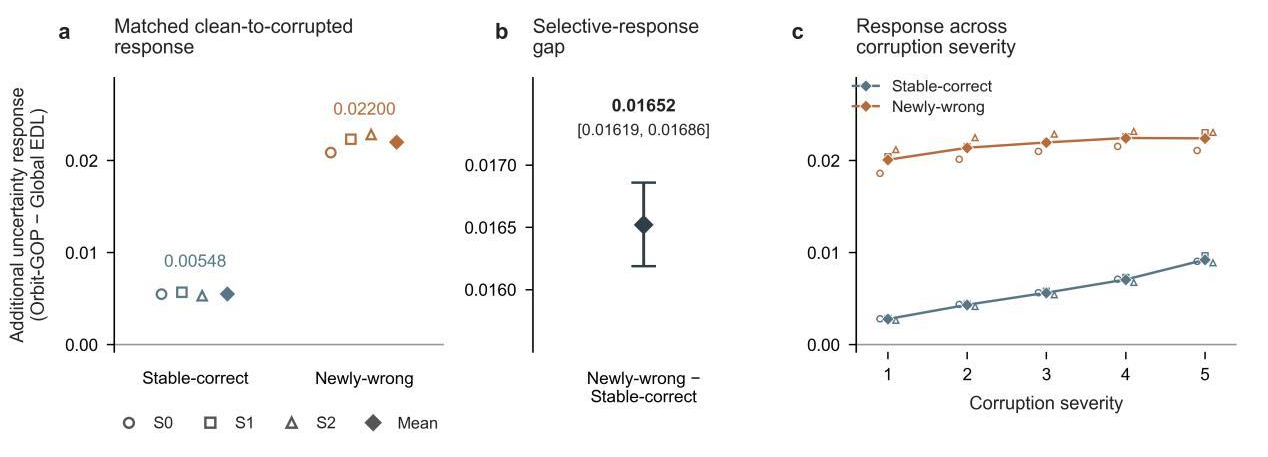
\includegraphics[width=\linewidth]{FigS1.png}\end{center}

\textbf{Repository Figure R1. Selective uncertainty responses under CIFAR-10-C covariate shifts.} (a) Additional uncertainty responses of Orbit-GOP relative to Global EDL, evaluated using matched clean-to-corrupted samples. Stable-correct denotes samples that are correctly classified under clean conditions and remain correct after corruption; Newly-wrong denotes samples that are correctly classified under clean conditions but become incorrect after corruption. Within each transition group, the additional response is defined as the clean-to-corrupted change in uncertainty for Orbit-GOP minus the corresponding change for Global EDL. S0--S2 denote the three fixed trained models, and diamonds indicate their arithmetic means. (b) Selective-response gap, defined as the additional response of Newly-wrong minus that of Stable-correct. The diamond indicates the point estimate, and the error bar represents the 95\% confidence interval obtained from 2,000 synchronized cluster-based sample-level bootstrap replicates. An expanded vertical scale is used to display the narrow interval. (c) Additional uncertainty responses of the two transition groups across the five corruption severity levels of CIFAR-10-C, covering all 15 corruption types. Symbols represent the three fixed trained models, and lines connect the three-model means as visual guides only. Panels (a) and (c) do not show error bars because separate group- and severity-specific confidence intervals were not retained in the finalized analysis artifacts. This analysis supports a larger additional response for Newly-wrong samples at the group-mean level, while Stable-correct samples retain a smaller positive response. It should therefore not be interpreted as a universal sample-level pattern or as a complete absence of response to stable-correct samples.

Aggregated over all corruption types and severity levels, the mean additional uncertainty responses are 0.0055 for Stable-correct and 0.0220 for Newly-wrong. The selective-response gap is 0.0165, with a 95\% cluster-bootstrap confidence interval of {[}0.0162, 0.0169{]}, supporting a stronger group-mean response of Orbit-GOP to samples that become incorrectly classified after corruption. This trend holds across all five corruption severity levels, with Newly-wrong retaining a higher mean additional response than Stable-correct even under mild corruption. However, the mean response of Stable-correct remains positive, and a small number of individual corruption--severity conditions exhibit differences in the opposite direction. The analysis therefore does not support absolute selectivity at either the individual-sample or individual-condition level.

\Needspace{8\baselineskip}
\section*{Repository Note R1. Protocol for inference efficiency and performance--cost analysis}\label{supplementary-note-s1.-protocol-for-inference-efficiency-and-performancecost-analysis}

\Needspace{6\baselineskip}
\subsection*{R1.1 Hardware and software environment}\label{s1.1-hardware-and-software-environment}

The end-to-end efficiency benchmarks in Table 8 and the view-configuration efficiency benchmarks in Fig. 9(b) were conducted in the same hardware and software environment. The GPU was an NVIDIA GeForce RTX 5060 Ti, and the CPU was an AMD Ryzen 5 9600X 6-Core Processor. The software environment comprised Windows-10-10.0.26200-SP0, Python 3.10.10, PyTorch 2.11.0+cu128, torchvision 0.26.0+cu128, and NumPy 1.26.4. The CUDA runtime reported by torch.version.cuda was 12.8, the cuDNN version code was 91900, and the NVIDIA driver version was 591.86. The model and GPU inputs used float32, with both automatic mixed precision and TF32 disabled. All efficiency experiments used the frozen ResNet18-EDL Seed-0 model. Orbit-GOP used Layer3, \emph{β} = 0.40, \emph{q}\textsubscript{func}-only risk, and the final decision-margin target and normalized generalized Jensen--Shannon divergence measure.

\Needspace{6\baselineskip}
\subsection*{R1.2 End-to-end latency and throughput}\label{s1.2-end-to-end-latency-and-throughput}

The efficiency benchmarks used a fixed input pool consisting of the first 2,048 images in the official CIFAR-10 test set. Image decoding, float32 conversion, mapping to {[}0, 1{]} before normalization, and preloading into pinned CPU memory were completed before timing. Disk reads and one-time preprocessing were therefore excluded from the reported latency. Batch = 1 and Batch = 64 indicate batches containing 1 and 64 base images, respectively. For multi-view Orbit-GOP, additional views are not counted separately toward the batch size.

For each method and batch-size setting, 50 warm-up iterations were followed by five repeated timing rounds. Each round contained 1,000 batches for Batch = 1 and 200 batches for Batch = 64. CUDA synchronization was performed immediately before and after the timed interval in each round, and wall-clock time was recorded using time.perf\_counter(). The mean batch latency in timing round \emph{r} is defined as

\begin{equation}
\begin{array}{r}
L_{r} = \frac{T_{r}}{I}
\end{array}
\label{eq:supp1}
\end{equation}

where \emph{T}\textsubscript{r} is the total wall-clock duration of the round expressed in milliseconds and \emph{I} is the number of batches in that round. Table 8 reports the arithmetic mean and sample standard deviation of the five \emph{L}\textsubscript{r} values. Throughput for Batch = 64 is calculated from the mean batch latency as

\begin{equation}
\begin{array}{r}
Throughput = \frac{1000B}{L}
\end{array}
\label{eq:supp2}
\end{equation}

where \emph{B} = 64 and \emph{L} is measured in ms/batch. Thus, throughput is not obtained from a separate independent benchmark.

\Needspace{6\baselineskip}
\subsection*{R1.3 Scope of end-to-end timing}\label{s1.3-scope-of-end-to-end-timing}

The timed interval includes batch selection from the fixed input pool, data transfer from pinned CPU memory to the GPU, mild-view construction, input normalization, network forward passes, method-specific gradient extraction, GOP functional-signature construction, Jensen--Shannon divergence computation, class-conditional reference lookup, empirical midrank mapping, evidence scaling, final uncertainty computation, result return, and finiteness checks.

Disk access, image decoding, model loading, one-time loading and sorting of the calibration reference, and fitting of \emph{c}\textsubscript{global} are excluded from the timed interval. All methods use the same frozen checkpoint, input pool, and deterministic batch order to reduce additional between-method variation caused by input scheduling.

\Needspace{6\baselineskip}
\subsection*{R1.4 Peak GPU memory}\label{s1.4-peak-gpu-memory}

Peak GPU memory is measured separately from latency. Before measuring each method and batch-size setting, CUDA synchronization, Python garbage collection, CUDA cache clearing, model-gradient clearing, and torch.cuda.reset\_peak\_memory\_stats() are performed in sequence. The method is then invoked once, and torch.cuda.max\_memory\_allocated() is read after CUDA synchronization.

Table 8 reports peak allocated memory for Batch = 64 in MiB. This quantity includes the memory occupied by the resident model itself. It is not equivalent to max\_memory\_reserved(), the additional workspace relative to the base model, or the total device memory usage displayed by nvidia-smi.

\Needspace{6\baselineskip}
\subsection*{R1.5 Stepwise computational profiling for Fig. 9(a)}\label{s1.5-stepwise-computational-profiling-for-fig.-10a}

The stepwise computational profile in Fig. 9(a) uses the final frozen Orbit-GOP configuration: ResNet18-EDL Seed-0, Layer3, Full Orbit, and \emph{β} = 0.40. At a batch size of 64, each timing mode begins with 50 warm-up batches, followed by five independent timing rounds of 200 batches each. The error ranges show the sample standard deviation of the five round-level mean latencies, rather than variation across individual batches, uncertainty across training seeds, or confidence intervals for detection performance.

The profiled steps are view construction, multi-view forward passes, gradient extraction, GOP functional-signature construction, Jensen--Shannon divergence computation, and risk mapping with evidence calibration. Each step is timed using its own CUDA synchronization boundaries. Risk mapping includes operations associated with returning results to the CPU, whereas some Python scheduling and surrounding control operations fall outside the six steps. The stepwise timings therefore describe the computational breakdown and cannot be directly summed to reconstruct the end-to-end inference latency reported in Table 8.

\Needspace{6\baselineskip}
\subsection*{R1.6 Performance--cost analysis for Fig. 9(b)}\label{s1.6-performancecost-analysis-for-fig.-10b}

Figure 9(b) compares the performance--cost relationships of three view configurations---Brightness-only, Reflect-shift-only, and Full Orbit---under the ResNet18-EDL Seed-0 development setting. All three configurations use Layer3, \emph{β} = 0.40, \emph{q}\textsubscript{func}-only calibration, the final decision margin, and normalized generalized Jensen--Shannon divergence.

Table 8 reports the inter-method efficiency benchmark, in which Orbit-GOP uses its frozen calibration reference. The latency measurements for Fig. 9(b) are obtained in a separate view-configuration benchmark. Each view configuration uses its own class-conditional reference constructed from the same CIFAR-10 calibration set, ensuring that its performance and latency measurements correspond to the same configuration. The corresponding development AUROC values are 0.87738508, 0.87766472, and 0.87842696 for Brightness-only, Reflect-shift-only, and Full Orbit, respectively. These results use only CIFAR-10 ID development and CIFAR-100 development data; they do not involve performance evaluation on official test sets, holdout data, or Tiny ImageNet. The Batch = 64 latencies are 32.44 $\pm$ 2.90 ms, 28.80 $\pm$ 0.01 ms, and 44.24 $\pm$ 1.28 ms for Brightness-only, Reflect-shift-only, and Full Orbit, respectively.

The error terms are the sample standard deviations of the means from five repeated timing rounds. Each pair of performance and cost coordinates is matched in checkpoint, functional layer, \emph{β}, risk definition, view set, and configuration-specific reference. Figure 9(b) presents only a descriptive performance--cost relationship under the development setting and is not used for statistical significance testing or cross-hardware Pareto claims.

\Needspace{6\baselineskip}
\subsection*{R1.7 Scope and limitations}\label{s1.7-scope-and-limitations}

These efficiency results reflect measurements obtained with the recorded hardware and software environment, the frozen Seed-0 model, and the fixed CIFAR-10 input pool. Although the environment, input order, and timing protocol are fully documented, GPU scheduling, thermal conditions, and background system load may still cause latency to vary between runs. We therefore do not claim exact numerical reproducibility of latency across different devices or execution environments. The efficiency analysis is also not intended to infer runtime-cost differences across training seeds.

\Needspace{8\baselineskip}
\section*{Repository Note R2. Base EDL training and global evidence calibration}\label{supplementary-note-s2.-base-edl-training-and-global-evidence-calibration}

\noindent\textbf{Protocol scope.} The historical training description in R2.1--R2.4 is retained for the existing S0--S2 results. The explicitly labeled confirmatory paragraphs state the frozen S3--S5 protocol; historical optimizer settings and fitted constants are not newly verified confirmatory facts.

\Needspace{6\baselineskip}
\subsection*{R2.1 Base EDL training objective}\label{s2.1-base-edl-training-objective}

All three base networks use the standard EDL parameterization. Let \emph{z}\textsubscript{k} denote the network output before Softplus. The class evidence and Dirichlet parameters are defined, respectively, as

\begin{equation}
\begin{array}{r}
e_{k} = Softplus(z_{k}),\alpha_{k} = e_{k} + 1
\end{array}
\label{eq:supp3}
\end{equation}

The sample-specific Dirichlet parameters are then constructed as

\begin{equation}
\begin{array}{r}
\alpha_{ik} = e_{ik} + 1,S_{i} = \sum_{k = 1}^{K}\alpha_{ik}
\end{array}
\label{eq:supp4}
\end{equation}

where \emph{K} = 10. The corresponding Dirichlet mean probabilities are

\begin{equation}
\begin{array}{r}
p_{ik} = \frac{\alpha_{ik}}{S_{i}}
\end{array}
\label{eq:supp5}
\end{equation}

The base EDL models use the Bayes risk under expected squared error. For a one-hot label \emph{y}\textsubscript{i}, the per-sample loss is

\begin{equation}
\begin{array}{r}
L_{risk}^{(i)} = \sum_{k = 1}^{K}\left\lbrack \left( y_{ik} - \frac{\alpha_{ik}}{S_{i}} \right)^{2} + \frac{\alpha_{ik}(S_{i} - \alpha_{ik})}{S_{i}^{2}(S_{i} + 1)} \right\rbrack
\end{array}
\label{eq:supp6}
\end{equation}

The first term measures the squared error between the Dirichlet mean probabilities and the ground-truth label, while the second term corresponds to the variance of the class probabilities under the Dirichlet distribution. To suppress spurious evidence for non-ground-truth classes, the label-masked Dirichlet parameters are constructed as

\begin{equation}
\begin{array}{r}
{\widetilde{\alpha}}_{i} = y_{i} + (1 - y_{i}) \odot \alpha_{i}
\end{array}
\label{eq:supp7}
\end{equation}

This fixes the Dirichlet parameter of the ground-truth class at 1 while retaining the original parameters of all other classes. The KL regularizer is defined as

\begin{equation}
\begin{array}{r}
L_{KL}^{(i)} = D_{KL}\left\lbrack Dir({\widetilde{\alpha}}_{i}) \parallel Dir(\mathbf{1}) \right\rbrack
\end{array}
\label{eq:supp8}
\end{equation}

At training epoch \emph{t}, the KL regularizer is linearly annealed over the first 10 epochs:

\begin{equation}
\begin{array}{r}
\lambda_{t} = \min\left( 1,\frac{t}{10} \right)
\end{array}
\label{eq:supp9}
\end{equation}

The overall training objective is therefore

\begin{equation}
\begin{array}{r}
L = \frac{1}{N_{b}}\sum_{i = 1}^{N_{b}}\left\lbrack L_{risk}^{(i)} + \lambda_{t}L_{KL}^{(i)} \right\rbrack
\end{array}
\label{eq:supp10}
\end{equation}

where \emph{N}\textsubscript{b} is the number of samples in the current mini-batch. Training does not use auxiliary OOD data, additional evidence constraints, or test-time adaptation. This loss formulation is consistent with the finalized training protocol of the frozen EDL baselines.

\Needspace{6\baselineskip}
\subsection*{R2.2 Optimization and training configuration}\label{s2.2-optimization-and-training-configuration}

\noindent\textbf{Frozen confirmatory checkpoint protocol.} ResNet18-EDL and VGG16-BN-EDL are specified to train for 200 epochs. Checkpoint selection uses the new 3,000-image Validation set, ordered by higher validation accuracy, then lower ECE\textsubscript{15}, then lower NLL, and finally earlier epoch. WRN-28-10-EDL uses the fixed epoch-200 checkpoint. Its 3,000-image Validation set is used only for diagnostics after epoch 200, not for checkpoint selection, early stopping, model admission, or seed replacement. Historical test-based admission described below is not part of this confirmatory checkpoint protocol.

\noindent\textbf{Confirmatory training recipe and completed checkpoints.} Each backbone was trained from scratch for 200 epochs for each of S3, S4 and S5, using batch size 128, SGD with momentum 0.9, Nesterov momentum and weight decay $5\times10^{-4}$. Initial learning rates were 0.1 for ResNet18 and WRN-28-10 and 0.01 for VGG16-BN. The frozen schedule used five warmup epochs followed by cosine decay to $10^{-6}$. Training retained the squared-error EDL Bayes risk and label-masked KL to the uniform Dirichlet, with coefficient $\min(1,e/10)$ for one-based epoch $e$. Augmentation comprised random $32\times32$ crops with padding 4 and random horizontal flips. The disjoint 44,000/3,000/3,000 Train/Validation/Calibration roles are specified in R2.3. Training used float16 CUDA convolution under AMP with FP32 Softplus and EDL loss; confirmatory inference precision is specified separately in Repository Note R4. The frozen selected epochs, in S3/S4/S5 order, were 198/200/200 for ResNet18, 184/200/191 for VGG16-BN and 200/200/200 for WRN-28-10. WRN validation was diagnostic only after training. The WRN S5 engineering retry restored standard GradScaler overflow recovery without changing the scientific configuration.

\noindent\textbf{Historical benchmark context.} The original protocol and results retained below describe the historical analyses. Their S0--S2 labels, data roles, fitted values, and resampling settings are not specifications or results for the S3--S5 confirmatory study.

All base models are trained from scratch without ImageNet-pretrained weights. ResNet18-EDL, VGG16-BN-EDL, and WRN-28-10-EDL are each trained for 200 epochs with a batch size of 128 using SGD, momentum of 0.9, Nesterov momentum enabled, and weight decay of 5 × 10\textsuperscript{−4}. The initial learning rate is 0.1 for ResNet18-EDL and WRN-28-10-EDL, and 0.01 for VGG16-BN-EDL.

A linear warm-up is applied during the first five epochs, followed by cosine learning-rate decay. Training augmentation consists only of random cropping and random horizontal flipping; Mixup, CutMix, label smoothing, auxiliary OOD samples, and test-time adaptation are not used. Three independent models, S0--S2, are trained for each backbone. After base-model training, all network parameters are frozen, and Orbit-GOP performs only inference-time functional analysis and evidence calibration.

The ResNet18-EDL backbone uses a CIFAR-adapted architecture with a 3×3, stride-1 first convolution and no initial max-pooling layer. The base model is trained using the EDL objective described above, without AGOP computations, cross-view orbit construction, or Orbit-GOP calibration.

\Needspace{6\baselineskip}
\subsection*{R2.3 Data partitioning and separation from parameter training}\label{s2.3-data-partitioning-and-separation-from-parameter-training}

\noindent\textbf{Frozen confirmatory data protocol.} The confirmatory study specifies seeds 3, 4, and 5 (S3--S5), with three independently trained models per backbone and nine models in total across ResNet18-EDL, VGG16-BN-EDL, and WRN-28-10-EDL. The 50,000 CIFAR-10 training images are partitioned by class-stratified sampling into 44,000 Train, 3,000 Validation, and 3,000 Calibration images, with 4,400/300/300 images per class. Train, Validation, and Calibration have mutually exclusive roles and disjoint samples. The official CIFAR-10 test set is excluded from training, checkpoint selection, and calibration.

\noindent\textbf{Historical benchmark context.} The original protocol and results retained below describe the historical analyses. Their S0--S2 labels, data roles, fitted values, and resampling settings are not specifications or results for the S3--S5 confirmatory study.

The original CIFAR-10 training set contains 50,000 samples. Under the final experimental protocol, 45,000 samples are used to train the base EDL parameters, while the remaining 5,000 are subsequently assigned to calibration and ID development: 3,000 samples for Orbit-GOP calibration and 2,000 for ID development. The 10,000 samples in the official CIFAR-10 test set are not used for model-parameter training.

Importantly, historical checkpoint selection for ResNet18-EDL and VGG16-BN-EDL used this 5,000-sample validation pool. Thus, although the final calibration and development sets do not overlap with the 45,000 samples used for model-parameter training, they cannot be considered fully independent of the model-selection process. Official CIFAR-10 test metrics also formed part of the WRN-28-10 training-admission gate. These limitations, earlier VGG test feedback, and reuse of the CIFAR-100 holdout subset are described in Section 4.1.2 of the main text. Freezing for a final run does not imply that the entire development process was independent of earlier test results.

\Needspace{6\baselineskip}
\subsection*{R2.4 Global evidence-scale calibration}\label{s2.4-global-evidence-scale-calibration}

\noindent\textbf{Frozen confirmatory Orbit-GOP configuration.} The calibration strength is $\beta=0.40$, and Full Orbit consists of Original, Brightness(0.9), and Reflect-shift. Functional responses are taken from ResNet18 Layer3, VGG16-BN Block4 before pool4, and WRN-28-10 Block3 before the final BN/ReLU. Calibration uses $n=3{,}000$ images from the separate Calibration subset.

\noindent\textbf{Historical calibration context.} The numerical scales listed below belong to the historical S0--S2 models. Newly fitted S3--S5 scales are reported separately in Repository Table R9.

After base-model training, the network parameters remain frozen. For each frozen model, a positive global evidence scale, \emph{c}\textsubscript{global} \textgreater{} 0, is fitted using the corresponding 3,000 CIFAR-10 calibration samples. This parameter adjusts only the overall evidence scale and does not update the classification network parameters.

Let \emph{e}\textsubscript{ik} denote the original class evidence for calibration sample \emph{i}, and let \emph{y}\textsubscript{i} denote its ground-truth class. The global scale is obtained by minimizing the classification negative log-likelihood on the calibration data:

\begin{equation}
\begin{array}{r}
c_{global} = \arg{\min_{c > 0}{- \frac{1}{N_{cal}}\sum_{i = 1}^{N_{cal}}{\log\left( \frac{1 + ce_{i,y_{i}}}{K + c\sum_{k = 1}^{K}e_{ik}} \right)}}}
\end{array}
\label{eq:supp11}
\end{equation}

where

\[N_{cal} = 3000\]

The Dirichlet parameters of Global EDL are consequently defined as

\begin{equation}
\begin{array}{r}
\alpha_{ik}^{global} = 1 + c_{global}e_{ik}
\end{array}
\label{eq:supp12}
\end{equation}

and its uncertainty is

\begin{equation}
\begin{array}{r}
u_{global}(x_{i}) = \frac{K}{K + c_{global}\sum_{k = 1}^{K}e_{ik}}
\end{array}
\label{eq:supp13}
\end{equation}

Because \emph{c}\textsubscript{global} \textgreater{} 0 and the same scaling is applied to the evidence of all classes for a given sample, global calibration preserves the ordering of the original class evidence. Global EDL therefore serves as the primary frozen EDL reference for Orbit-GOP. On top of this global scale, Orbit-GOP introduces a sample-specific evidence-retention factor determined by \emph{q}\textsubscript{func}. The global scale is fitted using only CIFAR-10 calibration data, without using formal near-OOD test samples.

Numerical fitting used c = exp(t) with t in {[}−8, 8{]}, bounded scalar minimization, xatol = 10\textsuperscript{−12}, and at most 1,000 iterations. In S0--S2 order, the retained \emph{c}\textsubscript{global} values are ResNet18: 16.661915817233986, 18.482690632268103, 24.498207644808492; VGG16-BN: 7.3263600911805815, 8.23366795313237, 8.241928951246619; WRN-28-10: 18.61084704601242, 15.044461840056668, 14.143128408532414. These are frozen calibration constants, not parameters refitted on the evaluation endpoints.

\Needspace{8\baselineskip}
\section*{Repository Note R3. Data preprocessing and view construction}\label{supplementary-note-s3.-data-preprocessing-and-view-construction}

\Needspace{6\baselineskip}
\subsection*{R3.1 Unified input preprocessing}\label{s3.1-unified-input-preprocessing}

All inputs for formal evaluation are ultimately converted to RGB tensors of shape 3 × 32 × 32. CIFAR-10 and CIFAR-100 retain their original resolution of 32 × 32 and are mapped to {[}0, 1{]} using ToTensor. All data are normalized using the CIFAR-10 statistics:

\emph{μ} = (0.4914, 0.4822, 0.4465), \emph{σ} = (0.2470, 0.2435, 0.2616).

Each channel is normalized according to

\begin{equation}
\begin{array}{r}
x_{c}' = \frac{x_{c} - \mu_{c}}{\sigma_{c}}
\end{array}
\label{eq:supp14}
\end{equation}

No random cropping or random flipping is used in the base test preprocessing. Method-specific stochastic views, including those used by C-EDL in the conditional analysis, are specified separately in Repository Note R5.2.

\Needspace{6\baselineskip}
\subsection*{R3.2 Tiny ImageNet preprocessing}\label{s3.2-tiny-imagenet-preprocessing}

Tiny ImageNet uses the OpenOOD evaluation list fixed in advance for the main experiments, containing 7,793 samples. All images are first converted to RGB, resized to 32 × 32 using bilinear interpolation, center-cropped to 32 × 32, and then converted to tensors in {[}0, 1{]}. After cross-view construction, all views are normalized using the CIFAR-10 mean and standard deviation specified above.

\Needspace{6\baselineskip}
\subsection*{R3.3 Supplementary evaluation data}\label{s3.3-supplementary-evaluation-data}

SVHN uses the official test split with three-channel 32 × 32 inputs. After tensor conversion, inputs are normalized in the same way as CIFAR-10. SVHN is used only for cross-domain OOD diagnostics.

CIFAR-10-C uses corrupted samples aligned with the indices of the official CIFAR-10 test set, covering 15 corruption types and five severity levels. Corrupted images are converted directly from the stored uint8 data to tensors in {[}0, 1{]}. The corruptions are not regenerated, and no denoising, test-time adaptation, or recalibration is performed.

\Needspace{6\baselineskip}
\subsection*{R3.4 Order of cross-view construction}\label{s3.4-order-of-cross-view-construction}

All mild views in Orbit-GOP are constructed before input normalization. For an original input in {[}0, 1{]}, the Brightness view is obtained by multiplying pixel values by 0.9 and clipping to {[}0, 1{]}. The Reflect-shift view is obtained by applying one-pixel reflection padding on all sides and then cropping the top-left 32 × 32 region, shifting the image content one pixel to the right and one pixel downward relative to the original view.

The Original, Brightness, and Reflect-shift views are constructed independently from the same original input, without composing the transformations. Each completed view is then normalized using the CIFAR-10 statistics before being passed to the frozen EDL model.

\Needspace{8\baselineskip}
\section*{Repository Note R4. Comparison methods and implementation settings}\label{supplementary-note-s4.-comparison-methods-and-implementation-settings}

\noindent\textbf{Confirmatory implementation.} All twelve methods in Table 2 are evaluated on the same frozen weights within each backbone/seed, across ResNet18, VGG16-BN and WRN-28-10 and S3--S5. Table 3 and Fig. 3 report the corresponding core-method ID results from these models. ReAct fits its 90th-percentile threshold (linear quantile interpolation) only to that model's new 3,000-image Calibration features. KNN and ViM use only that model's new 44,000-image Train features. KNN uses L2-normalized penultimate features and the exact 50th-neighbor Euclidean distance, retaining FP32 distance accumulation. The backbone dimensions and frozen ViM splits are:
\begin{center}
\begin{tabular}{lrrr}
\toprule
Backbone & Feature dimension $N$ & ViM split $D$ & Residual dimension $N-D$ \\
\midrule
ResNet18 & 512 & 256 & 256 \\
VGG16-BN & 512 & 256 & 256 \\
WRN-28-10 & 640 & 320 & 320 \\
\bottomrule
\end{tabular}
\end{center}
Here $D$ is the number of leading eigenvectors excluded from the residual basis: the implementation sorts eigenvalues in descending order and uses columns $D$ onward for $N_S$. ViM features are not L2-normalized. Model forward and gradient computations use FP32, with autocast and TF32 disabled; applicable calibration and offline score postprocessing use float64, with the frozen KNN FP32 exception above. Inference uses batches of 32 and two data-loader workers in fixed sample order. Each model/dataset extraction initializes NumPy RandomState(20260813) and passes the current batch to \texttt{transformed\_batch}; its transformation draws therefore follow these 32-image batches (including a final partial batch), not the historical 128-image logical batches. C-EDL uses frozen default C018 and fixed C009. C009 was selected in historical ResNet18/VGG16-BN development and transferred unchanged to WRN, with no confirmatory WRN tuning and no additional $c_{\mathrm{global}}$ multiplier. For confirmatory ID AURC, correctness compares each method's saved actual output prediction with the true ID label: Global EDL and Orbit-GOP inherit the base prediction, whereas C-EDL and ReAct can change predictions. AURC sorts risk in ascending order, breaks ties by original index and averages cumulative error fractions. OOD labels belong to a different class ontology; OOD classification accuracy and AURC are not applicable.

\noindent\textbf{Historical implementation and shared formulas.} The retained ResNet18 implementation descriptions below concern the historical S0--S2 setting; their 45,000-image feature bank, 512-dimensional features and historical view batches do not describe the confirmatory results in Tables 2 and 3. The method formulas remain applicable with the confirmatory settings above, except for the MSP additive offset specified in R4.1. Let z ∈ ℝ\textsuperscript{K} denote the network output before Softplus, let s = Softmax(z), and let h ∈ ℝ\textsuperscript{512} denote the historical ResNet18 feature vector after global average pooling and before the final classifier. Unless otherwise specified, all methods are evaluated with scores oriented so that larger values indicate a greater tendency toward OOD.

For OOD AUROC and FPR95, OOD is the positive class and larger scores indicate OOD. FPR95 uses the first empirical ROC point reaching at least 95\% OOD true-positive rate, including the complete tied-score block, without interpolation.

For the historical analyses using the base-model error indicator, including Table 7, selective risk uses that frozen indicator, sorts uncertainty in ascending order with source index as the secondary key, and computes AURC as the arithmetic mean of cumulative risks at all retained-sample counts. NLL averages the negative natural logarithm of the true-class Dirichlet probability clipped to {[}10\textsuperscript{−15}, 1{]}; the Brier score averages the sum of squared class-probability errors. ECE15 uses 15 equal-width bins of maximum Dirichlet probability, weighted absolute confidence--accuracy differences, left-closed and right-open bins, and a closed upper edge for the final bin. Correctness in this historical analysis uses the frozen base prediction. Table 7 averages separately computed metrics equally over its 225 conditions.

\Needspace{6\baselineskip}
\subsection*{R4.1 Output-based baselines}\label{s4.1-output-based-baselines}

MSP uses the Softmax probabilities computed from the raw logits of the frozen model. The confirmatory implementation in Table 2 saves $1-\max_k s_k(x)$. Across all 18 confirmatory backbone--seed--near-OOD comparisons, the saved MSP scores have a tied block at zero; under the frozen empirical ROC rule, the first point reaching at least 95\% OOD true-positive rate includes this block at a threshold of zero, yielding both a true-positive rate and FPR95 of 1. This describes the saved-score threshold behavior and does not establish the cause of the zero-score ties. The historical formula below differs only by an additive constant of one in real arithmetic; this notation difference does not imply an error in the saved AUROC or FPR95. The retained historical score is defined as

\begin{equation}
\begin{array}{r}
S_{MSP}(x) = - \max_{k}s_{k}(x)
\end{array}
\label{eq:supp15}
\end{equation}

Predictive Entropy likewise uses the Softmax probabilities of the raw logits and is computed using natural logarithms:

\begin{equation}
\begin{array}{r}
S_{Ent}(x) = - \sum_{k = 1}^{K}s_{k}(x)\log s_{k}(x)
\end{array}
\label{eq:supp16}
\end{equation}

Energy is constructed directly from the logits before Softplus:

\begin{equation}
\begin{array}{r}
S_{Energy}(x) = - T\log{\sum_{k = 1}^{K}{\exp\left( \frac{z_{k}(x)}{T} \right)}}
\end{array}
\label{eq:supp17}
\end{equation}

We fix \emph{T} = 1 and perform no additional energy fine-tuning.

Importantly, these Softmax probabilities are computed from the raw logits rather than using the Dirichlet mean probabilities of EDL.

\Needspace{6\baselineskip}
\subsection*{R4.2 Feature-based baselines}\label{s4.2-feature-based-baselines}

In the historical ResNet18 setting, ReAct-Energy uses the 512-dimensional features after global average pooling and before the classifier; confirmatory feature dimensions and reference roles are given at the start of Repository Note R4. Given the frozen classifier \emph{z} = \emph{Wh} + \emph{b}, features are first clipped from above at threshold \emph{τ}:

\begin{equation}
\begin{array}{r}
\widetilde{h} = \min(h,\tau)
\end{array}
\label{eq:supp18}
\end{equation}

The logits are then recomputed from the clipped features, and the Energy score is calculated with \emph{T} = 1. The threshold \emph{τ} is estimated using only the 3,000 CIFAR-10 calibration samples for the corresponding frozen model and is set to the 90th percentile of all calibration feature elements. No OOD development data are used to fit the threshold.

Historical ResNet18 KNN uses the same 512-dimensional penultimate features. Each feature vector is first L2-normalized, and a fixed ID feature bank is constructed from the 45,000 CIFAR-10 samples used for parameter training. For each test sample, Euclidean distances to the feature bank are computed, and the distance to the 50th nearest neighbor is used as the OOD score. Thus, \emph{k} is fixed at 50, with no additional search over \emph{k}.

Historical ResNet18 ViM also uses the 512-dimensional penultimate features, but without L2 normalization. Let \emph{W} and \emph{b} denote the parameters of the final classification layer. We first define

\begin{equation}
\begin{array}{r}
u = - W^{\dagger}b
\end{array}
\label{eq:supp19}
\end{equation}

and construct the residual subspace from the 45,000 CIFAR-10 training feature vectors. The residual-subspace dimension is fixed at \emph{D} = 256. Denoting its basis by \emph{N}\textsubscript{S}, the ViM score is defined as

\begin{equation}
\begin{array}{r}
S_{ViM}(x) = a\left\| (h(x) - u)N_{S} \right\|_{2} - logsumexp(z(x))
\end{array}
\label{eq:supp20}
\end{equation}

where the scaling coefficient \emph{a} is fitted using only the CIFAR-10 training-feature statistics of the corresponding frozen model, without using OOD test samples.

\Needspace{6\baselineskip}
\subsection*{R4.3 Gradient-based baselines}\label{s4.3-gradient-based-baselines}

The following GAIA-Z and GradNorm formulas are shared by the historical and confirmatory implementations; confirmatory weights and precision follow the settings at the start of Repository Note R4. GAIA-Z uses gradients with respect to the outputs of all BatchNorm2d layers in the network. For each input, the gradient target is the maximum raw logit:

\begin{equation}
\begin{array}{r}
t(x) = \max_{k}z_{k}(x)
\end{array}
\label{eq:supp21}
\end{equation}

Let \emph{g}\textsubscript{ℓqrs} denote the gradient for channel \emph{q} of BatchNorm layer \emph{ℓ}. We first compute the spatial fraction of locations with nonzero gradients in that channel:

\begin{equation}
\begin{array}{r}
a_{\ell q}(x) = \frac{1}{H_{\ell}W_{\ell}}\sum_{r,s}^{}\mathbf{1}\left\lbrack g_{\ell qrs} \neq 0 \right\rbrack
\end{array}
\label{eq:supp22}
\end{equation}

The GAIA-Z score is then obtained by squaring and averaging the responses across BatchNorm channels. We use the Z variant for the CIFAR setting, without additional layer selection or threshold search.

GradNorm computes per-sample gradient norms at the final classifier. Let

\begin{equation}
\begin{array}{r}
L(x) = - \sum_{k = 1}^{K}{\log{s_{k}(x)}}
\end{array}
\label{eq:supp23}
\end{equation}

and let \emph{W} denote the final classifier weights. The OOD score used in this study is

\begin{equation}
\begin{array}{r}
S_{GradNorm}(x) = - \sum_{k,j}^{}\left| \frac{\partial L(x)}{\partial W_{kj}} \right|
\end{array}
\label{eq:supp24}
\end{equation}

The gradient norm is the elementwise L1 sum over the classifier weight matrix and excludes bias gradients. Computation is performed separately for each sample, with \emph{T} = 1 and no additional parameter tuning.

\Needspace{6\baselineskip}
\subsection*{R4.4 C-EDL}\label{s4.4-c-edl}

C-EDL is adapted from the public implementation in the GitHub repository \url{https://github.com/team-daniel/cedl} at commit \texttt{c939f279\allowbreak{}6065f448\allowbreak{}bf307789\allowbreak{}1c6a4b34\allowbreak{}2a424101} to the same frozen EDL base models as Orbit-GOP. The formal comparison follows the executable evidence-based semantics: conflict is computed from the five view-specific evidence vectors, their mean evidence is multiplied by exp(−δC), and one is then added to obtain the adjusted Dirichlet parameters. This differs from directly scaling the aggregated Dirichlet parameters in the paper equations. The OOD score is K divided by the adjusted total Dirichlet strength. The authors' default parameters are T = 5, \emph{β}\textsubscript{conflict} = 1.5, λ = 0.5, and δ = 1. The historical filtering references for Fig. 5 remain separately specified in Repository Note R5.2.

For each of the historical ResNet18 and VGG16-BN backbones only, development tuning evaluated all 36 combinations of \emph{β}\textsubscript{conflict} ∈ \{1.0, 1.5, 2.0\}, λ ∈ \{0.25, 0.50, 0.75\}, and δ ∈ \{0.5, 1.0, 1.5, 2.0\}, with T = 5 fixed. Selection maximized mean AUROC across S0--S2 on 2,000 CIFAR-10 ID-development and 12,500 CIFAR-100 development samples. Ties at six decimal places were resolved by lower mean FPR95, lower mean ID prediction-change rate, smaller normalized Euclidean distance from the default parameters, and finally ascending lexicographic parameter order. The distance normalized \emph{β}\textsubscript{conflict}, λ, and δ by 0.5, 0.25, and 0.5, respectively. One configuration was shared across seeds for each backbone.

The historical ResNet18/VGG16-BN view generator used random state 20260813, batches of 128, and the rotation, vertical circular-shift, and Gaussian-noise distributions described in R5.2; transformation draws depended on this batch order. Formal VGG16-BN forward and gradient computations used FP32 with autocast and TF32 disabled, and offline conflict and metric reductions used float64. Both backbones selected the following frozen parameters:

\emph{T} = 5, \emph{β}\textsubscript{conflict} = 1.0, \emph{λ} = 0.75, \emph{δ} = 0.5.

The reported final runs use the frozen C-EDL configurations. This run-level freezing should be distinguished from the earlier test access and adaptive Orbit-GOP development described in Section 4.1.2. C-EDL and Orbit-GOP operate on the same frozen models, but C-EDL does not impose the explicit prediction-preserving constraint defined for Orbit-GOP in Section 3.5.

\Needspace{8\baselineskip}
\section*{Repository Note R5. Protocols for mechanistic analyses}\label{supplementary-note-s5.-protocols-for-mechanistic-analyses}

The analyses below use frozen EDL models but differ in their diagnostic data subsets and reference configurations. The supervised probes in R5.1 are auxiliary diagnostic models, not components of the Orbit-GOP inference rule.

\Needspace{6\baselineskip}
\subsection*{R5.1 Controlled functional-instability diagnostics}\label{s5.1-controlled-functional-instability-diagnostics}

The diagnostics in Fig. 4 used three frozen ResNet18-EDL models trained with seeds 0, 1 and 2. Functional responses were obtained from the 256-channel output of layer3. The three views were the original image, an image multiplied by 0.9 and clipped to {[}0, 1{]}, and a one-pixel rightward and downward shift implemented by reflection padding. View transformations preceded input normalization. The reference class was the original-view prediction and remained fixed across views.

For each view, gradients of the raw-logit margin \(z_{c} - log\sum_{k \neq c}^{}\exp z_{k}\) were taken with respect to layer3. The spatial mean of the squared gradient in each channel was normalized across all channels after adding \(10^{- 12}\). Functional discrepancy \(d_{GOP}\) was the generalized Jensen--Shannon divergence of the three signatures divided by \(\log 3\). Functional risk \(q_{\text{func}}\) used the empirical midrank of \(d_{GOP}\) within the original-predicted-class reference distribution from 3,000 CIFAR-10 calibration images, separately for each model. Figure 4(a) used risk records for all 10,000 official CIFAR-10 test images, all 10,000 official CIFAR-100 test images, all 26,032 official SVHN test images, and the fixed OpenOOD evaluation list of 7,793 Tiny ImageNet images, separately for each model. CIFAR-10 images were grouped by original-prediction correctness. Symbols and horizontal bars denote model-specific medians and interquartile ranges. The displayed density curves were obtained from 512 equal-width bins on {[}0, 1{]}, smoothed with a Gaussian kernel of standard deviation 0.04 using reflection at the boundaries and truncation at four standard deviations, and averaged equally across models. For Tiny ImageNet, functional-risk records were recovered from the stored Global EDL and function-only uncertainty scores by inverting the evidence-retention relation with the historical coefficient 0.20; they were not newly computed from gradients for this plot.

Figures 4(b) and 4(c) used a separate diagnostic split. CIFAR-10 contributed 1,000 calibration and 4,000 analysis images, and CIFAR-100 contributed 5,000 calibration and 10,000 analysis images, all from their training splits. For each model, the high-evidence threshold was the median original EDL uncertainty among correctly classified CIFAR-10 diagnostic calibration images. Original uncertainty was \(u_{0} = 10/\sum_{k}^{}\alpha_{k}\), with \(\alpha_{k} = softplus\left( z_{k} \right) + 1\). Correctly classified CIFAR-10 images formed the negative class and CIFAR-100 images formed the positive class; both classes were restricted to \(u_{0} \leq \tau_{50}\). The seed-specific thresholds were 0.1942606270, 0.1911670119 and 0.1921216846. The resulting calibration class counts were 462/216, 463/226 and 467/209, and the analysis class counts were 1,909/407, 1,856/407 and 1,922/375, respectively, with ID/OOD counts reported in that order.

For uncertainty stratification, the retained ID and OOD diagnostic calibration samples were pooled within each model to estimate the 20th, 40th, 60th and 80th percentiles of \(u_{0}\). These fixed boundaries defined five analysis strata, with internal boundaries assigned to the lower stratum. A stratum contributed only when both classes contained at least 30 samples. Its AUROC was weighted by \(\min\left( n_{ID},n_{OOD} \right)\), normalized over eligible strata. At least three eligible strata were required, and the sum of these minimum class counts had to be at least 200. Model-specific stratified AUROCs were averaged equally across the three models.

The control probe used \(\left( u_{0},d_{prob},d_{feat},d_{grad} \right)\), and the extended probe additionally used \(d_{GOP}\). The output-change measure \(d_{prob}\) was the generalized Jensen--Shannon divergence, divided by \(\log 3\), of the three 10-class Dirichlet mean probability vectors. The feature measure \(d_{feat}\) averaged cosine distances over all three view pairs using spatially averaged layer3 features. Each feature norm was floored at \(10^{- 12}\) before L2 normalization. The gradient measure \(d_{grad}\) was the population standard deviation across views of \(\log\left( \parallel g^{(v)} \parallel_{2} + 10^{- 12} \right)\), where \(g^{(v)}\) is the full layer3 gradient of the fixed-class decision margin. The gradient was not normalized before computing its norm. Both probes used the same calibration and analysis samples. Each pipeline fitted a StandardScaler followed by logistic regression on the diagnostic calibration samples, including both ID and OOD examples. Logistic regression explicitly used L2 regularization, \(C = 1\), the liblinear solver, balanced class weights, a maximum of 1,000 iterations and random state 20260805. Analysis AUROC used the predicted probability of the OOD class. The original scikit-learn version could not be recovered from the retained diagnostic records; only explicitly recorded hyperparameters are reported.

The confidence intervals for the three-model means in Fig. 4(b, c) were obtained using 2,000 synchronous bootstrap replicates. Calibration and analysis samples were resampled separately with replacement within dataset-by-source-class groups. The same sampled source positions were used for all three frozen models and both probes. Both scalers and logistic regressions were refitted within each replicate; the uncertainty threshold and stratum boundaries remained fixed. Eligible strata and their weights were determined from the resampled class counts. The three model-specific statistics were averaged within each replicate, and the 2.5th and 97.5th percentiles defined the intervals.

\Needspace{6\baselineskip}
\subsection*{R5.2 Conditional residual-ranking analysis}\label{s5.2-conditional-residual-ranking-analysis}

Figure 5 retained the historical conflict-reference parameters, with separate view sets for the two filtering conditions described below. ResNet18 analyses compared 2,000 CIFAR-10 development images with 12,500 CIFAR-100 holdout images. VGG16-BN analyses used 10,000 CIFAR-10 test images, 10,000 CIFAR-100 test images and 7,793 Tiny ImageNet images. Each backbone used three frozen models. VGG16-BN functional risk was taken from the final Block4 records; filtering quantities were retained from the historical reference records and matched by model seed, dataset and source index. The CIFAR-100 holdout subset had been accessed in earlier project stages; the fixed rules of this conditional analysis therefore provide a run-specific separation from fitting, not evidence that the holdout was never previously examined.

\begin{sloppypar}
Let \(e_{kv}\) denote raw output evidence. Intra-class conflict was the class mean of \({std}_{v}\left( e_{kv} \right)/\left( {mean}_{v}\left( e_{kv} \right) + 10^{- 8} \right)\), using population standard deviations. For each view and class pair \(i < j\), the inter-class contribution was
\end{sloppypar}

\begin{equation}
\begin{array}{r}
w_{ijv} = 2\frac{\min\left( e_{iv},e_{jv} \right)}{\max\left( e_{iv},e_{jv} \right)}\frac{\min\left( e_{iv},e_{jv} \right)}{\sum_{k}^{}e_{kv}}
\end{array}
\label{eq:supp25}
\end{equation}

\begin{sloppypar}
Zero-denominator terms were set to zero. Inter-class conflict was the view mean of \(1 - exp\left\lbrack - 1.5\sqrt{\sum_{i < j}^{}w_{ijv}^{2}} \right\rbrack\). Total conflict was
\end{sloppypar}

\begin{equation}
\begin{array}{r}
C = clip\left( C_{inter} + C_{intra} - C_{inter}C_{intra} - 0.5\left( C_{inter} - C_{intra} \right)^{2},0,1 \right)
\end{array}
\label{eq:supp26}
\end{equation}

For \(q_{conf}\), these quantities used the original, brightness and reflection-shift views. Total conflict was mapped to an empirical midrank within the original-predicted-class reference distribution of 3,000 CIFAR-10 calibration images, separately for each model. The low-conflict analysis retained ID and OOD images satisfying \(q_{conf} \leq 0.2\).

C-EDL uncertainty used a distinct five-view configuration: the original view and four random transformed views. Transform types were rotation, vertical circular shift or Gaussian noise. Rotation angles were sampled from \(\left\lbrack - 15^{\circ},15^{\circ} \right\rbrack\), with linear interpolation and replicated borders; vertical circular shifts were sampled as integers from \(- 2\) through \(1\); Gaussian noise had standard deviation 0.01. Transformed pixel values were clipped to {[}0, 1{]}. The historical implementation used transform random state 20260813. Transform types were drawn for each batch before drawing the individual transformation parameters; the retained VGG16-BN reference run used batches of 128 images. It computed conflict from these five evidence vectors, multiplied their mean evidence by \(\exp( - C)\), added one to form Dirichlet parameters and returned \(10/\sum_{k}^{}\alpha_{k}\). The configuration was \(T = 5\), conflict coefficient 1.5, disagreement penalty 0.5 and decay coefficient 1.0.

For the C-EDL-unflagged analysis, each model's threshold was the 95th percentile of its own CIFAR-10 calibration uncertainty, estimated by linear quantile interpolation. Both ID and OOD images with uncertainty at or below this threshold were retained. These historical thresholds were not replaced by the later development-tuned C-EDL configuration. Both conditional analyses evaluated only \(q_{\text{func}}\), with OOD as the positive class, and averaged the three model-specific AUROCs equally. Counts before and after filtering are reported in Repository Table R4.

Confidence intervals used 5,000 synchronous bootstrap replicates with random seed 20260817. ID images were resampled with replacement, CIFAR-100 images were resampled within source classes, and Tiny ImageNet images were resampled at the image level. Within each backbone's analysis, source draws were shared across its three models and both filtering conditions. Fixed conditions were applied within each replicate; reference distributions, thresholds and models were not refitted. Percentile intervals were obtained from the replicate-wise means of the three model AUROCs.

\Needspace{8\baselineskip}
\textbf{Repository Table R4. Sample counts for the conditional analyses in Fig. 5.}

\begingroup
\small
\setlength{\tabcolsep}{3.5pt}
\renewcommand{\arraystretch}{1.13}
\setlength{\LTpre}{3pt}
\setlength{\LTpost}{3pt}
\begin{longtable}[]{@{}
  >{\raggedright\arraybackslash}p{(\linewidth - 10\tabcolsep) * \real{0.1322}}
  >{\raggedright\arraybackslash}p{(\linewidth - 10\tabcolsep) * \real{0.1552}}
  >{\centering\arraybackslash}p{(\linewidth - 10\tabcolsep) * \real{0.0862}}
  >{\centering\arraybackslash}p{(\linewidth - 10\tabcolsep) * \real{0.2098}}
  >{\centering\arraybackslash}p{(\linewidth - 10\tabcolsep) * \real{0.2012}}
  >{\centering\arraybackslash}p{(\linewidth - 10\tabcolsep) * \real{0.2155}}@{}}
\toprule\noalign{}
\begin{minipage}[b]{\linewidth}\raggedright
\textbf{Backbone}
\end{minipage} & \begin{minipage}[b]{\linewidth}\raggedright
\textbf{Near-OOD data}
\end{minipage} & \begin{minipage}[b]{\linewidth}\centering
\textbf{Model}
\end{minipage} & \begin{minipage}[b]{\linewidth}\centering
\textbf{Before filtering}
\end{minipage} & \begin{minipage}[b]{\linewidth}\centering
\textbf{Low conflict}
\end{minipage} & \begin{minipage}[b]{\linewidth}\centering
\textbf{C-EDL unflagged}
\end{minipage} \\
\midrule\noalign{}
\endhead
\bottomrule\noalign{}
\endlastfoot
ResNet18 & CIFAR-100 & S0 & 2,000 / 12,500 & 435 / 382 & 1,907 / 7,778 \\
ResNet18 & CIFAR-100 & S1 & 2,000 / 12,500 & 372 / 357 & 1,888 / 7,901 \\
ResNet18 & CIFAR-100 & S2 & 2,000 / 12,500 & 404 / 345 & 1,901 / 7,954 \\
VGG16-BN & CIFAR-100 & S0 & 10,000 / 10,000 & 2,112 / 233 & 9,447 / 6,431 \\
VGG16-BN & CIFAR-100 & S1 & 10,000 / 10,000 & 1,950 / 208 & 9,476 / 6,304 \\
VGG16-BN & CIFAR-100 & S2 & 10,000 / 10,000 & 2,012 / 239 & 9,475 / 6,314 \\
VGG16-BN & Tiny ImageNet & S0 & 10,000 / 7,793 & 2,112 / 126 & 9,447 / 4,631 \\
VGG16-BN & Tiny ImageNet & S1 & 10,000 / 7,793 & 1,950 / 117 & 9,476 / 4,523 \\
VGG16-BN & Tiny ImageNet & S2 & 10,000 / 7,793 & 2,012 / 126 & 9,475 / 4,595 \\
\end{longtable}
\endgroup

\begingroup\footnotesize
Note. Each count pair is ID / OOD. Low conflict denotes \(q_{conf} \leq 0.2\); C-EDL unflagged denotes uncertainty at or below the model-specific calibration Q95. The two conditions are applied separately to the same original samples. For VGG16-BN, the CIFAR-10 ID samples are also shared across the two near-OOD comparisons.\par
\endgroup

\Needspace{6\baselineskip}
\subsection*{R5.3 Sample-level ranking and case visualization}\label{s5.3-sample-level-ranking-and-case-visualization}

The analyses in Figs. 6 and 7 used the frozen ResNet18-EDL models. For each near-OOD image \(o\), the ranking percentile of method \(m\) was

\begin{equation}
\begin{array}{r}
R_{m}(o) = \frac{N_{m,less}(o) + \frac{1}{2}N_{m,tie}(o)}{10,000}
\end{array}
\label{eq:supp27}
\end{equation}

where \(N_{m,less}(o)\) and \(N_{m,tie}(o)\) count reference ID scores strictly below and equal to \(s_{m}(o)\), respectively. The reference consisted of all 10,000 official CIFAR-10 test images evaluated by the same model and method. These percentiles are descriptive evaluation statistics, distinct from the calibration reference used to compute functional risk. Ranking change was \(\Delta R = R_{Orbit} - R_{Global}\), using the formal Orbit configuration with \(\beta = 0.40\). The heatmaps in Fig. 6(a) used \(q_{\text{func}}\) and the Global EDL uncertainty percentile as their axes. Both axes used fixed boundaries \(0,0.2,0.4,0.6,0.8,1\), with left-closed, right-open bins except that the final bin included one. Functional-risk bin assignments were retained from the saved formal records. Within each two-dimensional bin and dataset, the displayed mean pooled the sample records from all three models. Thus, the mean weights each model according to its number of records in that bin rather than averaging the three bin means equally. Bins with fewer than 30 records from any one model were hatched; these records remained in the means and descriptive contribution summaries.

The eight fixed cases were selected retrospectively from historical CIFAR-100 test and Tiny ImageNet evaluation records, rather than specified before inspecting ranking outcomes. For each dataset, positive candidates were required to have positive historical Joint-minus-Global ranking changes for all three models, and the two candidates with the largest mean changes were selected. Negative candidates were required to have negative changes for all three models, and the two candidates with the smallest mean changes were selected. The historical Joint variant used \(\beta = 0.20\) and risk \(q_{\text{func}}q_{evi}\); the auxiliary score \(q_{evi}\) belonged to that exploratory variant and is not used in the final function-only method. The selected identities were locked before visualization replay and retained without reselection when annotations were updated to the final function-only results with \(\beta = 0.40\). Figure 7 displayed the first selected case from each dataset and sign group. Repository Table R5 specifies all eight identities; these fixed identities, rather than a new application of the historical selector, define the displayed case set. Because selection used ranking outcomes, the cases are illustrative and are not an unbiased sample of the evaluation population.

Channel heatmaps used the frozen seed-0 functional signatures, whereas \(q_{\text{func}}\) and \(\Delta R\) annotations were means over the three models. For each case and model, channels were ranked by the mean normalized signature across the original, brightness and reflection-shift views. The 20 largest channels were selected, and all three views shared this channel set and order. The displayed values were entries of the full 256-channel normalized signatures; they were not renormalized after selecting 20 channels. The displayed heatmaps used a shared linear color scale from 0 to 0.045. Channel ranks were defined within each case and did not imply shared channel identities across cases.

\Needspace{15\baselineskip}
\textbf{Repository Table R5. Fixed case identities used in Figs. 6(b) and 7.}

\begingroup
\small
\setlength{\tabcolsep}{3.5pt}
\renewcommand{\arraystretch}{1.13}
\begin{longtable}[]{@{}
  >{\raggedright\arraybackslash}p{(\linewidth - 6\tabcolsep) * \real{0.2012}}
  >{\raggedright\arraybackslash}p{(\linewidth - 6\tabcolsep) * \real{0.2931}}
  >{\centering\arraybackslash}p{(\linewidth - 6\tabcolsep) * \real{0.2299}}
  >{\centering\arraybackslash}p{(\linewidth - 6\tabcolsep) * \real{0.2759}}@{}}
\toprule\noalign{}
\begin{minipage}[b]{\linewidth}\raggedright
\textbf{Dataset}
\end{minipage} & \begin{minipage}[b]{\linewidth}\raggedright
\textbf{Historical selection group}
\end{minipage} & \begin{minipage}[b]{\linewidth}\centering
\textbf{Zero-based index}
\end{minipage} & \begin{minipage}[b]{\linewidth}\centering
\textbf{Shown in Fig. 7}
\end{minipage} \\
\midrule\noalign{}
\endhead
\bottomrule\noalign{}
\endlastfoot
CIFAR-100 & Positive & 3769 & Yes \\
CIFAR-100 & Positive & 2320 & No \\
CIFAR-100 & Negative & 1271 & Yes \\
CIFAR-100 & Negative & 1969 & No \\
Tiny ImageNet & Positive & 4374 & Yes \\
Tiny ImageNet & Positive & 7779 & No \\
Tiny ImageNet & Negative & 2887 & Yes \\
Tiny ImageNet & Negative & 2946 & No \\
\end{longtable}
\endgroup

\begingroup\footnotesize
Note. All eight cases are included in Fig. 6(b). CIFAR-100 indices refer to the official test-set ordering; Tiny ImageNet indices refer to the fixed evaluation manifest. Positive and negative identify the sign groups used by the historical selector, not a newly applied selection rule. The Tiny ImageNet images at indices 4374, 7779, 2887 and 2946 are val\_5614.JPEG, val\_9979.JPEG, val\_3709.JPEG and val\_3787.JPEG, respectively.\par
\endgroup

\Needspace{8\baselineskip}
\section*{Repository Note R6. Fixed-configuration evaluation on additional samples}\label{supplementary-note-s6.-fixed-configuration-evaluation-on-additional-samples}

\noindent\textbf{Historical benchmark context.} The original protocol and results retained below describe the historical analyses. Their S0--S2 labels, data roles, fitted values, and resampling settings are not specifications or results for the S3--S5 confirmatory study.

\Needspace{6\baselineskip}
\subsection*{R6.1 Purpose, data eligibility, and historical scope}\label{s6.1-purpose-data-eligibility-and-historical-scope}

This evaluation examined the incremental effect of Orbit-GOP relative to Global EDL after the selected models and method configurations had been fixed. Development-tuned C-EDL was retained as a separate related-method comparison. It used 1,994 eligible CIFAR-10.1 v6 images as additional same-class ID data and 968 Tiny ImageNet images as OOD data. The same sample identities were evaluated by all three methods on each of the three existing ResNet18-EDL and three existing VGG16-BN-EDL models. The 2,962 unique identities must not be multiplied by the number of models and treated as independent observations.

CIFAR-10.1 v6 was obtained from the author GitHub repository {\def\UrlBreaks{\do\/\do\.\do\-\do\a\do\b\do\c\do\d\do\e\do\f\do\g\do\h\do\i\do\j\do\k\do\l\do\m\do\n\do\o\do\p\do\q\do\r\do\s\do\t\do\u\do\v\do\w\do\x\do\y\do\z}\url{https://github.com/modestyachts/CIFAR-10.1}} at commit \texttt{d9982abb\allowbreak{}0bfc4846\allowbreak{}b8d13a11\allowbreak{}e66b887d\allowbreak{}946205d0}; the original data and label arrays were retained unchanged. The dataset and its Tiny Images provenance are cited in main-text References \textsuperscript{{[}39,40{]}}. Of the original 2,000 images, zero-based index 105 was excluded as a same-source counterpart of candidate 96, which was retained by the prespecified index rule. Indices 117, 760, and 945 were excluded because their same-source counterparts belonged to the frozen CIFAR-10 training subset. Indices 1026 and 1999 were conservatively excluded before new-sample inference because a common source with training images could not be ruled out; these two cases were not classified as confirmed duplicates. No replacement images were added. Results therefore refer to an eligibility-screened subset, not the unfiltered standard v6 test set.

The OOD set consists of positions 32--999 in the fixed 1,000-image OpenOOD val\_tin list, using zero-based positions. The first 32 images had previously undergone technical inference and were excluded. The remaining 968 identities are disjoint from the 7,793-image Tiny ImageNet list used in the original benchmark evaluation; none of the previously excluded or unassigned images was restored, and no Tiny training or unlabeled test images were added. The included set spans 20 annotated classes. Category eligibility was checked against the prespecified CIFAR-10 overlap rules; this does not constitute scene-level relabeling or a claim that all categories were previously unseen.

Duplicate screening compared candidate identities and pixel hashes against the available CIFAR-10, CIFAR-100, and Tiny ImageNet source collections and the new v6 data. A complete search at the fixed 64-bit dHash Hamming threshold of four was followed by visual review of flagged pairs. This procedure does not guarantee detection of every cropped, rotated, or edited counterpart. The available project run, session, and command records did not reveal prior experimental use of the retained candidate identities; missing or unrecorded history cannot be excluded. Eligibility decisions, execution settings, and sample order were fixed before this evaluation. ID followed ascending original v6 indices; OOD followed the original manifest order. Neither performance nor prediction difficulty was used to choose or replace images.

\Needspace{6\baselineskip}
\subsection*{R6.2 Frozen models and numerical execution}\label{s6.2-frozen-models-and-numerical-execution}

All six existing checkpoints, class-conditioned reference distributions, and global scales were reused without training, fitting, or parameter search. Orbit-GOP used the function-only risk, β = 0.40, Layer3 for ResNet18 and Block4 for VGG16-BN, and the original, brightness-0.9, and one-pixel right/down reflection-shift views. The raw-logit margin used the class predicted from the original view as the fixed gradient target. The C-EDL configuration remained T = 5, \emph{β}\textsubscript{conflict} = 1.0, λ = 0.75, and δ = 0.5, using the evidence-based implementation described in R4.4 without an additional global scale.

Preprocessing followed Repository Note R3: v6 retained its native 32 × 32 resolution, whereas Tiny images were converted to RGB and resized with bilinear interpolation to 32 × 32. Views were constructed before normalization. Computation used the recorded RTX 5060 Ti / PyTorch 2.11.0+cu128 / CUDA 12.8 environment, FP32 forwards and feature gradients, and disabled autocast and TF32. ResNet18 used computation microbatches of 32; VGG16-BN retained the FP32 implementation with batches of 128. All methods shared the same original-view forward products within a model. ResNet18 Global EDL and Orbit-GOP retained the existing float64 evidence recovery from float32 Dirichlet probabilities and strength, with negative rounding residuals clipped at zero; C-EDL retained direct Softplus evidence. VGG16-BN retained direct FP32 Softplus evidence and the existing P13 class-conditioned reference. The ResNet reference retained its recorded construction from original prediction/evidence and functional-response records; it was not refitted to enforce a newly matched batch history.

C-EDL view construction retained CPU NumPy RandomState(20260813), reset for each backbone, model seed, and data domain, with logical transformation batches of 128 in fixed sample order. For each of four transformed views, transformation types were drawn for the full logical batch before the per-image rotation, vertical circular-shift, or Gaussian-noise parameters described in R5.2. The completed tensors were then split into ResNet microbatches of at most 32 without redrawing transformations; VGG retained computation batches of 128. The original view was reused rather than recalculated in another batch. Reference lookup, score reductions, and statistics used float64. This shared-original-view scheduling was validated on old development/technical samples before new-sample inference and is not claimed to be bitwise identical to the original formal evaluation schedule.

\Needspace{6\baselineskip}
\subsection*{R6.3 Evaluation and paired statistical analysis}\label{s6.3-evaluation-and-paired-statistical-analysis}

OOD is the positive class and larger scores indicate OOD. AUROC gives tied scores their standard average-rank contribution. FPR95 uses the first empirical ROC point attaining at least 95\% OOD true-positive rate, with the complete tied-score block included and no interpolation. Each method is evaluated separately for S0--S2, and the arithmetic mean is reported within each backbone. The primary difference is Orbit-GOP minus Global EDL; the secondary difference is Orbit-GOP minus development-tuned C-EDL. Positive AUROC differences and negative FPR95 differences favor Orbit-GOP.

The 95\% percentile intervals use 5,000 synchronized paired sample-bootstrap replicates. ID and OOD are both resampled within their true classes, preserving the retained size of each class. A NumPy Generator with PCG64 seed 20260912 draws ID classes 0--9 first, followed by OOD classes in lexicographic identifier order. The same sampled positions are used for all methods, seeds, and backbones. Within each replicate, the paired difference is computed for each fixed model and then averaged equally across the three seeds of the relevant backbone. The 2.5th and 97.5th percentiles use linear quantile interpolation. Point estimates come from the complete retained samples, not the bootstrap means. Models, calibration references, and scales are not refitted. This two-domain class-stratified scheme is specific to the additional-sample evaluation and does not replace the resampling protocols of the original figures or tables.

All eight preselected backbone-by-comparison-by-metric intervals and all per-seed results are reported. The intervals condition on the fixed models, configurations, and represented class composition; they do not account for the full training-randomness population, previously unobserved classes, or the adaptive development history. Intervals containing zero are not evidence of equivalence. No claim of simultaneous multiple-comparison significance is made.

\Needspace{6\baselineskip}
\subsection*{R6.4 Results and interpretation}\label{s6.4-results-and-interpretation}

main-text Table 4 gives the three-seed means, Table R6b retains every per-seed result, and Supplementary Table S3 reports all mean paired differences with their intervals. Relative to Global EDL, Orbit-GOP improves both metrics for each of the six models, with all four backbone-level mean intervals in the favorable direction. Relative to C-EDL, ResNet18 AUROC is lower for every seed and its mean paired interval is unfavorable; the FPR95 interval includes zero. For VGG16-BN, the mean FPR95 interval favors Orbit-GOP, while the AUROC interval includes zero. VGG seed 2 is unfavorable to Orbit-GOP on both metrics relative to C-EDL. The findings therefore support incremental ranking information beyond global evidence scaling but not a universal advantage over cross-view evidential calibration.

\Needspace{6\baselineskip}
\noindent Former Table S6a is now main-text Table 4 (historical additional-sample means).

\subsection*{Repository Table R6b. Additional-sample results for every fixed model.}\label{supplementary-table-s6b.-additional-sample-results-for-every-fixed-model.}

\begingroup
\small
\setlength{\tabcolsep}{3.5pt}
\renewcommand{\arraystretch}{1.13}
\begin{longtable}[]{@{}
  >{\raggedright\arraybackslash}p{(\linewidth - 8\tabcolsep) * \real{0.1649}}
  >{\raggedright\arraybackslash}p{(\linewidth - 8\tabcolsep) * \real{0.0701}}
  >{\centering\arraybackslash}p{(\linewidth - 8\tabcolsep) * \real{0.3577}}
  >{\centering\arraybackslash}p{(\linewidth - 8\tabcolsep) * \real{0.2030}}
  >{\centering\arraybackslash}p{(\linewidth - 8\tabcolsep) * \real{0.2044}}@{}}
\toprule\noalign{}
\begin{minipage}[b]{\linewidth}\raggedright
\textbf{Backbone}
\end{minipage} & \begin{minipage}[b]{\linewidth}\raggedright
\textbf{Seed}
\end{minipage} & \begin{minipage}[b]{\linewidth}\centering
\textbf{Method}
\end{minipage} & \begin{minipage}[b]{\linewidth}\centering
\textbf{AUROC ↑}
\end{minipage} & \begin{minipage}[b]{\linewidth}\centering
\textbf{FPR95 ↓}
\end{minipage} \\
\midrule\noalign{}
\endhead
\bottomrule\noalign{}
\endlastfoot
ResNet18 & S0 & Global EDL & 0.812122 & 0.604814 \\
ResNet18 & S0 & C-EDL Dev-tuned & 0.824066 & 0.555667 \\
ResNet18 & S0 & Orbit-GOP & 0.815840 & 0.563691 \\
ResNet18 & S1 & Global EDL & 0.799158 & 0.612337 \\
ResNet18 & S1 & C-EDL Dev-tuned & 0.809919 & 0.560682 \\
ResNet18 & S1 & Orbit-GOP & 0.802612 & 0.565697 \\
ResNet18 & S2 & Global EDL & 0.812558 & 0.593781 \\
ResNet18 & S2 & C-EDL Dev-tuned & 0.818059 & 0.561685 \\
ResNet18 & S2 & Orbit-GOP & 0.816662 & 0.552658 \\
VGG16-BN & S0 & Global EDL & 0.789330 & 0.709127 \\
VGG16-BN & S0 & C-EDL Dev-tuned & 0.798961 & 0.648445 \\
VGG16-BN & S0 & Orbit-GOP & 0.800926 & 0.571715 \\
VGG16-BN & S1 & Global EDL & 0.800097 & 0.693079 \\
VGG16-BN & S1 & C-EDL Dev-tuned & 0.810238 & 0.600301 \\
VGG16-BN & S1 & Orbit-GOP & 0.812078 & 0.543129 \\
VGG16-BN & S2 & Global EDL & 0.791040 & 0.699097 \\
VGG16-BN & S2 & C-EDL Dev-tuned & 0.804494 & 0.559679 \\
VGG16-BN & S2 & Orbit-GOP & 0.801917 & 0.562688 \\
\end{longtable}
\endgroup

\begingroup\footnotesize
Note. No seed or method has been omitted. These rows are repeated evaluations of the same sample identities, not independent expansions of the test set. Metric definitions and direction are as in R6.3.\par
\endgroup

\Needspace{6\baselineskip}
\Needspace{16\baselineskip}
\noindent Former Table S6c is now journal Supplementary Table S3 (all eight historical paired comparisons).

\subsection*{R6.5 Execution checks and evidence limits}\label{s6.5-execution-checks-and-evidence-limits}

The full evaluation and its score lock were completed before comparative analysis. Saved identities, batch order, random-state records, finite scores, probability constraints, signatures, CDF mapping, score formulas, and reported metric reductions were checked. Following completion of the 24 ResNet18 S0 logical batches, an event-logging error interrupted the terminal model-state report. The saved batches were verified by identity and hash and reused without repeated inference. The original S0 terminal in-memory state hash was not persisted; a recovery-process check does not replace that missing first-run record. The corresponding terminal parameter and BatchNorm state records were persisted for the other five models.

This is an additional-sample fixed-configuration evaluation, not a claim of preregistration, wholly new categories, or unconditional independence. Earlier test feedback, holdout reuse, and model-selection dependencies described in main-text Section 4.1.2 remain part of the study history. The new data and execution schedule also differ from the original benchmark runs, so between-evaluation changes in absolute metrics are not isolated method effects. No raw images were uploaded or redistributed for this evaluation; data provenance and usage documentation are distinct from code licensing, and no new external image-data permission was obtained.

\clearpage
\section*{Repository Table R7. Complete confirmatory results for all 12 methods}\label{tab:s7}
All values use S3--S5. AUROC and FPR95 are proportions; ID AURC is in $10^{-3}$ units. Accuracy and prediction changes are percentages. Mean rows report sample SD ($ddof=1$). OOD classification accuracy and OOD AURC are not applicable and are not computed.
\subsection*{ResNet18 / CIFAR100}
\begingroup
\footnotesize
\setlength{\tabcolsep}{3pt}
\renewcommand{\arraystretch}{1.1}
\begin{longtable}{@{}llccc@{}}
\toprule
Method & Seed & AUROC & FPR95 & Change (\%) \\
\midrule
\endhead
\bottomrule
\endlastfoot
MSP & S3 & 0.8509 & 1.0000 & 0.00 \\
MSP & S4 & 0.8544 & 1.0000 & 0.00 \\
MSP & S5 & 0.8501 & 1.0000 & 0.00 \\
MSP & Mean $\pm$ SD & $0.8518 \pm 0.0022$ & $1.0000 \pm 0.0000$ & $0.00 \pm 0.00$ \\
Predictive Entropy & S3 & 0.8697 & 0.4719 & 0.00 \\
Predictive Entropy & S4 & 0.8737 & 0.4454 & 0.00 \\
Predictive Entropy & S5 & 0.8691 & 0.4721 & 0.00 \\
Predictive Entropy & Mean $\pm$ SD & $0.8708 \pm 0.0025$ & $0.4631 \pm 0.0154$ & $0.00 \pm 0.00$ \\
Energy & S3 & 0.8696 & 0.4684 & 0.00 \\
Energy & S4 & 0.8738 & 0.4470 & 0.00 \\
Energy & S5 & 0.8689 & 0.4725 & 0.00 \\
Energy & Mean $\pm$ SD & $0.8708 \pm 0.0027$ & $0.4626 \pm 0.0137$ & $0.00 \pm 0.00$ \\
ReAct-Energy & S3 & 0.8364 & 0.6548 & 0.41 \\
ReAct-Energy & S4 & 0.8485 & 0.6153 & 0.52 \\
ReAct-Energy & S5 & 0.8352 & 0.6486 & 1.02 \\
ReAct-Energy & Mean $\pm$ SD & $0.8400 \pm 0.0073$ & $0.6396 \pm 0.0212$ & $0.65 \pm 0.33$ \\
KNN & S3 & 0.8366 & 0.4837 & 0.00 \\
KNN & S4 & 0.8394 & 0.4752 & 0.00 \\
KNN & S5 & 0.8346 & 0.4950 & 0.00 \\
KNN & Mean $\pm$ SD & $0.8369 \pm 0.0024$ & $0.4846 \pm 0.0099$ & $0.00 \pm 0.00$ \\
ViM & S3 & 0.8587 & 0.4986 & 0.00 \\
ViM & S4 & 0.8623 & 0.4816 & 0.00 \\
ViM & S5 & 0.8537 & 0.5443 & 0.00 \\
ViM & Mean $\pm$ SD & $0.8583 \pm 0.0043$ & $0.5082 \pm 0.0324$ & $0.00 \pm 0.00$ \\
GAIA-Z & S3 & 0.8148 & 0.6840 & 0.00 \\
GAIA-Z & S4 & 0.8124 & 0.6557 & 0.00 \\
GAIA-Z & S5 & 0.7930 & 0.7484 & 0.00 \\
GAIA-Z & Mean $\pm$ SD & $0.8067 \pm 0.0120$ & $0.6960 \pm 0.0475$ & $0.00 \pm 0.00$ \\
GradNorm & S3 & 0.8544 & 0.5551 & 0.00 \\
GradNorm & S4 & 0.8713 & 0.4716 & 0.00 \\
GradNorm & S5 & 0.8607 & 0.5210 & 0.00 \\
GradNorm & Mean $\pm$ SD & $0.8621 \pm 0.0085$ & $0.5159 \pm 0.0420$ & $0.00 \pm 0.00$ \\
Global EDL & S3 & 0.8696 & 0.4693 & 0.00 \\
Global EDL & S4 & 0.8739 & 0.4466 & 0.00 \\
Global EDL & S5 & 0.8690 & 0.4729 & 0.00 \\
Global EDL & Mean $\pm$ SD & $0.8708 \pm 0.0027$ & $0.4629 \pm 0.0143$ & $0.00 \pm 0.00$ \\
C-EDL (C018) & S3 & 0.8751 & 0.4141 & 14.29 \\
C-EDL (C018) & S4 & 0.8787 & 0.4078 & 14.59 \\
C-EDL (C018) & S5 & 0.8742 & 0.4121 & 14.56 \\
C-EDL (C018) & Mean $\pm$ SD & $0.8760 \pm 0.0024$ & $0.4113 \pm 0.0032$ & $14.48 \pm 0.17$ \\
C-EDL (C009) & S3 & 0.8757 & 0.4079 & 14.29 \\
C-EDL (C009) & S4 & 0.8799 & 0.4028 & 14.59 \\
C-EDL (C009) & S5 & 0.8753 & 0.4125 & 14.56 \\
C-EDL (C009) & Mean $\pm$ SD & $0.8770 \pm 0.0025$ & $0.4077 \pm 0.0049$ & $14.48 \pm 0.17$ \\
Orbit-GOP & S3 & 0.8765 & 0.3995 & 0.00 \\
Orbit-GOP & S4 & 0.8789 & 0.3927 & 0.00 \\
Orbit-GOP & S5 & 0.8752 & 0.4133 & 0.00 \\
Orbit-GOP & Mean $\pm$ SD & $0.8769 \pm 0.0019$ & $0.4018 \pm 0.0105$ & $0.00 \pm 0.00$ \\
\end{longtable}
\endgroup

\clearpage
\subsection*{ResNet18 / Tiny}
\begingroup
\footnotesize
\setlength{\tabcolsep}{3pt}
\renewcommand{\arraystretch}{1.1}
\begin{longtable}{@{}llccc@{}}
\toprule
Method & Seed & AUROC & FPR95 & Change (\%) \\
\midrule
\endhead
\bottomrule
\endlastfoot
MSP & S3 & 0.8748 & 1.0000 & 0.00 \\
MSP & S4 & 0.8760 & 1.0000 & 0.00 \\
MSP & S5 & 0.8723 & 1.0000 & 0.00 \\
MSP & Mean $\pm$ SD & $0.8744 \pm 0.0019$ & $1.0000 \pm 0.0000$ & $0.00 \pm 0.00$ \\
Predictive Entropy & S3 & 0.8912 & 0.3783 & 0.00 \\
Predictive Entropy & S4 & 0.8926 & 0.3545 & 0.00 \\
Predictive Entropy & S5 & 0.8898 & 0.3690 & 0.00 \\
Predictive Entropy & Mean $\pm$ SD & $0.8912 \pm 0.0014$ & $0.3673 \pm 0.0120$ & $0.00 \pm 0.00$ \\
Energy & S3 & 0.8912 & 0.3754 & 0.00 \\
Energy & S4 & 0.8931 & 0.3537 & 0.00 \\
Energy & S5 & 0.8894 & 0.3702 & 0.00 \\
Energy & Mean $\pm$ SD & $0.8912 \pm 0.0019$ & $0.3664 \pm 0.0113$ & $0.00 \pm 0.00$ \\
ReAct-Energy & S3 & 0.8651 & 0.5765 & 0.67 \\
ReAct-Energy & S4 & 0.8763 & 0.5445 & 0.60 \\
ReAct-Energy & S5 & 0.8616 & 0.5827 & 1.07 \\
ReAct-Energy & Mean $\pm$ SD & $0.8677 \pm 0.0077$ & $0.5679 \pm 0.0205$ & $0.78 \pm 0.25$ \\
KNN & S3 & 0.8462 & 0.4020 & 0.00 \\
KNN & S4 & 0.8504 & 0.3947 & 0.00 \\
KNN & S5 & 0.8473 & 0.4041 & 0.00 \\
KNN & Mean $\pm$ SD & $0.8479 \pm 0.0022$ & $0.4003 \pm 0.0049$ & $0.00 \pm 0.00$ \\
ViM & S3 & 0.8757 & 0.4067 & 0.00 \\
ViM & S4 & 0.8782 & 0.4073 & 0.00 \\
ViM & S5 & 0.8707 & 0.4479 & 0.00 \\
ViM & Mean $\pm$ SD & $0.8749 \pm 0.0038$ & $0.4206 \pm 0.0236$ & $0.00 \pm 0.00$ \\
GAIA-Z & S3 & 0.8480 & 0.5624 & 0.00 \\
GAIA-Z & S4 & 0.8523 & 0.5265 & 0.00 \\
GAIA-Z & S5 & 0.8295 & 0.6846 & 0.00 \\
GAIA-Z & Mean $\pm$ SD & $0.8433 \pm 0.0121$ & $0.5912 \pm 0.0829$ & $0.00 \pm 0.00$ \\
GradNorm & S3 & 0.8826 & 0.4240 & 0.00 \\
GradNorm & S4 & 0.8939 & 0.3668 & 0.00 \\
GradNorm & S5 & 0.8864 & 0.4338 & 0.00 \\
GradNorm & Mean $\pm$ SD & $0.8876 \pm 0.0057$ & $0.4082 \pm 0.0362$ & $0.00 \pm 0.00$ \\
Global EDL & S3 & 0.8912 & 0.3754 & 0.00 \\
Global EDL & S4 & 0.8933 & 0.3538 & 0.00 \\
Global EDL & S5 & 0.8895 & 0.3705 & 0.00 \\
Global EDL & Mean $\pm$ SD & $0.8913 \pm 0.0019$ & $0.3666 \pm 0.0113$ & $0.00 \pm 0.00$ \\
C-EDL (C018) & S3 & 0.8946 & 0.3442 & 17.44 \\
C-EDL (C018) & S4 & 0.8982 & 0.3287 & 16.31 \\
C-EDL (C018) & S5 & 0.8924 & 0.3489 & 17.23 \\
C-EDL (C018) & Mean $\pm$ SD & $0.8951 \pm 0.0029$ & $0.3406 \pm 0.0106$ & $16.99 \pm 0.60$ \\
C-EDL (C009) & S3 & 0.8951 & 0.3406 & 17.44 \\
C-EDL (C009) & S4 & 0.8990 & 0.3266 & 16.31 \\
C-EDL (C009) & S5 & 0.8935 & 0.3419 & 17.23 \\
C-EDL (C009) & Mean $\pm$ SD & $0.8959 \pm 0.0028$ & $0.3364 \pm 0.0085$ & $16.99 \pm 0.60$ \\
Orbit-GOP & S3 & 0.8959 & 0.3417 & 0.00 \\
Orbit-GOP & S4 & 0.8972 & 0.3311 & 0.00 \\
Orbit-GOP & S5 & 0.8942 & 0.3392 & 0.00 \\
Orbit-GOP & Mean $\pm$ SD & $0.8958 \pm 0.0015$ & $0.3373 \pm 0.0055$ & $0.00 \pm 0.00$ \\
\end{longtable}
\endgroup

\clearpage
\subsection*{ResNet18 / ID}
\begingroup
\footnotesize
\setlength{\tabcolsep}{3pt}
\renewcommand{\arraystretch}{1.1}
\begin{longtable}{@{}llccc@{}}
\toprule
Method & Seed & AURC ($10^{-3}$) & Accuracy (\%) & Change (\%) \\
\midrule
\endhead
\bottomrule
\endlastfoot
MSP & S3 & 11.087 & 92.88 & 0.00 \\
MSP & S4 & 11.240 & 93.43 & 0.00 \\
MSP & S5 & 11.278 & 93.06 & 0.00 \\
MSP & Mean $\pm$ SD & $11.202 \pm 0.102$ & $93.12 \pm 0.28$ & $0.00 \pm 0.00$ \\
Predictive Entropy & S3 & 8.504 & 92.88 & 0.00 \\
Predictive Entropy & S4 & 8.812 & 93.43 & 0.00 \\
Predictive Entropy & S5 & 7.892 & 93.06 & 0.00 \\
Predictive Entropy & Mean $\pm$ SD & $8.403 \pm 0.468$ & $93.12 \pm 0.28$ & $0.00 \pm 0.00$ \\
Energy & S3 & 8.518 & 92.88 & 0.00 \\
Energy & S4 & 8.826 & 93.43 & 0.00 \\
Energy & S5 & 7.932 & 93.06 & 0.00 \\
Energy & Mean $\pm$ SD & $8.426 \pm 0.454$ & $93.12 \pm 0.28$ & $0.00 \pm 0.00$ \\
ReAct-Energy & S3 & 12.660 & 92.82 & 0.08 \\
ReAct-Energy & S4 & 11.787 & 93.41 & 0.06 \\
ReAct-Energy & S5 & 12.156 & 93.12 & 0.09 \\
ReAct-Energy & Mean $\pm$ SD & $12.201 \pm 0.438$ & $93.12 \pm 0.30$ & $0.08 \pm 0.02$ \\
KNN & S3 & 10.387 & 92.88 & 0.00 \\
KNN & S4 & 10.614 & 93.43 & 0.00 \\
KNN & S5 & 9.814 & 93.06 & 0.00 \\
KNN & Mean $\pm$ SD & $10.272 \pm 0.412$ & $93.12 \pm 0.28$ & $0.00 \pm 0.00$ \\
ViM & S3 & 10.280 & 92.88 & 0.00 \\
ViM & S4 & 9.763 & 93.43 & 0.00 \\
ViM & S5 & 9.352 & 93.06 & 0.00 \\
ViM & Mean $\pm$ SD & $9.798 \pm 0.465$ & $93.12 \pm 0.28$ & $0.00 \pm 0.00$ \\
GAIA-Z & S3 & 21.322 & 92.88 & 0.00 \\
GAIA-Z & S4 & 18.895 & 93.43 & 0.00 \\
GAIA-Z & S5 & 22.679 & 93.06 & 0.00 \\
GAIA-Z & Mean $\pm$ SD & $20.965 \pm 1.917$ & $93.12 \pm 0.28$ & $0.00 \pm 0.00$ \\
GradNorm & S3 & 11.015 & 92.88 & 0.00 \\
GradNorm & S4 & 9.560 & 93.43 & 0.00 \\
GradNorm & S5 & 10.123 & 93.06 & 0.00 \\
GradNorm & Mean $\pm$ SD & $10.233 \pm 0.734$ & $93.12 \pm 0.28$ & $0.00 \pm 0.00$ \\
Global EDL & S3 & 8.522 & 92.88 & 0.00 \\
Global EDL & S4 & 8.836 & 93.43 & 0.00 \\
Global EDL & S5 & 7.945 & 93.06 & 0.00 \\
Global EDL & Mean $\pm$ SD & $8.434 \pm 0.452$ & $93.12 \pm 0.28$ & $0.00 \pm 0.00$ \\
C-EDL (C018) & S3 & 8.746 & 92.72 & 2.11 \\
C-EDL (C018) & S4 & 8.814 & 93.17 & 2.60 \\
C-EDL (C018) & S5 & 8.050 & 92.68 & 2.59 \\
C-EDL (C018) & Mean $\pm$ SD & $8.537 \pm 0.423$ & $92.86 \pm 0.27$ & $2.43 \pm 0.28$ \\
C-EDL (C009) & S3 & 8.710 & 92.72 & 2.11 \\
C-EDL (C009) & S4 & 8.789 & 93.17 & 2.60 \\
C-EDL (C009) & S5 & 8.069 & 92.68 & 2.59 \\
C-EDL (C009) & Mean $\pm$ SD & $8.523 \pm 0.395$ & $92.86 \pm 0.27$ & $2.43 \pm 0.28$ \\
Orbit-GOP & S3 & 8.391 & 92.88 & 0.00 \\
Orbit-GOP & S4 & 8.160 & 93.43 & 0.00 \\
Orbit-GOP & S5 & 7.680 & 93.06 & 0.00 \\
Orbit-GOP & Mean $\pm$ SD & $8.077 \pm 0.363$ & $93.12 \pm 0.28$ & $0.00 \pm 0.00$ \\
\end{longtable}
\endgroup

\clearpage
\subsection*{VGG16-BN / CIFAR100}
\begingroup
\footnotesize
\setlength{\tabcolsep}{3pt}
\renewcommand{\arraystretch}{1.1}
\begin{longtable}{@{}llccc@{}}
\toprule
Method & Seed & AUROC & FPR95 & Change (\%) \\
\midrule
\endhead
\bottomrule
\endlastfoot
MSP & S3 & 0.8084 & 1.0000 & 0.00 \\
MSP & S4 & 0.8090 & 1.0000 & 0.00 \\
MSP & S5 & 0.8099 & 1.0000 & 0.00 \\
MSP & Mean $\pm$ SD & $0.8091 \pm 0.0008$ & $1.0000 \pm 0.0000$ & $0.00 \pm 0.00$ \\
Predictive Entropy & S3 & 0.8446 & 0.6334 & 0.00 \\
Predictive Entropy & S4 & 0.8441 & 0.6738 & 0.00 \\
Predictive Entropy & S5 & 0.8487 & 0.6303 & 0.00 \\
Predictive Entropy & Mean $\pm$ SD & $0.8458 \pm 0.0025$ & $0.6458 \pm 0.0243$ & $0.00 \pm 0.00$ \\
Energy & S3 & 0.8455 & 0.6257 & 0.00 \\
Energy & S4 & 0.8454 & 0.6639 & 0.00 \\
Energy & S5 & 0.8493 & 0.6213 & 0.00 \\
Energy & Mean $\pm$ SD & $0.8467 \pm 0.0023$ & $0.6370 \pm 0.0234$ & $0.00 \pm 0.00$ \\
ReAct-Energy & S3 & 0.8363 & 0.6676 & 0.86 \\
ReAct-Energy & S4 & 0.8357 & 0.7088 & 1.09 \\
ReAct-Energy & S5 & 0.8393 & 0.6428 & 0.64 \\
ReAct-Energy & Mean $\pm$ SD & $0.8371 \pm 0.0019$ & $0.6731 \pm 0.0333$ & $0.86 \pm 0.23$ \\
KNN & S3 & 0.8388 & 0.5148 & 0.00 \\
KNN & S4 & 0.8393 & 0.5585 & 0.00 \\
KNN & S5 & 0.8402 & 0.5744 & 0.00 \\
KNN & Mean $\pm$ SD & $0.8394 \pm 0.0007$ & $0.5492 \pm 0.0309$ & $0.00 \pm 0.00$ \\
ViM & S3 & 0.8443 & 0.5118 & 0.00 \\
ViM & S4 & 0.8458 & 0.5196 & 0.00 \\
ViM & S5 & 0.8473 & 0.5208 & 0.00 \\
ViM & Mean $\pm$ SD & $0.8458 \pm 0.0015$ & $0.5174 \pm 0.0049$ & $0.00 \pm 0.00$ \\
GAIA-Z & S3 & 0.8453 & 0.5348 & 0.00 \\
GAIA-Z & S4 & 0.8660 & 0.4936 & 0.00 \\
GAIA-Z & S5 & 0.8570 & 0.5196 & 0.00 \\
GAIA-Z & Mean $\pm$ SD & $0.8561 \pm 0.0104$ & $0.5160 \pm 0.0208$ & $0.00 \pm 0.00$ \\
GradNorm & S3 & 0.8391 & 0.6890 & 0.00 \\
GradNorm & S4 & 0.8356 & 0.7421 & 0.00 \\
GradNorm & S5 & 0.8414 & 0.6798 & 0.00 \\
GradNorm & Mean $\pm$ SD & $0.8387 \pm 0.0029$ & $0.7036 \pm 0.0336$ & $0.00 \pm 0.00$ \\
Global EDL & S3 & 0.8455 & 0.6257 & 0.00 \\
Global EDL & S4 & 0.8455 & 0.6638 & 0.00 \\
Global EDL & S5 & 0.8493 & 0.6215 & 0.00 \\
Global EDL & Mean $\pm$ SD & $0.8468 \pm 0.0022$ & $0.6370 \pm 0.0233$ & $0.00 \pm 0.00$ \\
C-EDL (C018) & S3 & 0.8574 & 0.4850 & 13.22 \\
C-EDL (C018) & S4 & 0.8597 & 0.4851 & 13.77 \\
C-EDL (C018) & S5 & 0.8615 & 0.4651 & 13.26 \\
C-EDL (C018) & Mean $\pm$ SD & $0.8596 \pm 0.0021$ & $0.4784 \pm 0.0115$ & $13.42 \pm 0.31$ \\
C-EDL (C009) & S3 & 0.8579 & 0.4958 & 13.22 \\
C-EDL (C009) & S4 & 0.8598 & 0.5034 & 13.77 \\
C-EDL (C009) & S5 & 0.8623 & 0.4777 & 13.26 \\
C-EDL (C009) & Mean $\pm$ SD & $0.8600 \pm 0.0022$ & $0.4923 \pm 0.0132$ & $13.42 \pm 0.31$ \\
Orbit-GOP & S3 & 0.8631 & 0.4354 & 0.00 \\
Orbit-GOP & S4 & 0.8658 & 0.4457 & 0.00 \\
Orbit-GOP & S5 & 0.8686 & 0.4189 & 0.00 \\
Orbit-GOP & Mean $\pm$ SD & $0.8659 \pm 0.0028$ & $0.4333 \pm 0.0135$ & $0.00 \pm 0.00$ \\
\end{longtable}
\endgroup

\clearpage
\subsection*{VGG16-BN / Tiny}
\begingroup
\footnotesize
\setlength{\tabcolsep}{3pt}
\renewcommand{\arraystretch}{1.1}
\begin{longtable}{@{}llccc@{}}
\toprule
Method & Seed & AUROC & FPR95 & Change (\%) \\
\midrule
\endhead
\bottomrule
\endlastfoot
MSP & S3 & 0.8357 & 1.0000 & 0.00 \\
MSP & S4 & 0.8348 & 1.0000 & 0.00 \\
MSP & S5 & 0.8399 & 1.0000 & 0.00 \\
MSP & Mean $\pm$ SD & $0.8368 \pm 0.0027$ & $1.0000 \pm 0.0000$ & $0.00 \pm 0.00$ \\
Predictive Entropy & S3 & 0.8699 & 0.5095 & 0.00 \\
Predictive Entropy & S4 & 0.8667 & 0.5769 & 0.00 \\
Predictive Entropy & S5 & 0.8738 & 0.5056 & 0.00 \\
Predictive Entropy & Mean $\pm$ SD & $0.8701 \pm 0.0036$ & $0.5307 \pm 0.0401$ & $0.00 \pm 0.00$ \\
Energy & S3 & 0.8711 & 0.5009 & 0.00 \\
Energy & S4 & 0.8682 & 0.5677 & 0.00 \\
Energy & S5 & 0.8745 & 0.5021 & 0.00 \\
Energy & Mean $\pm$ SD & $0.8713 \pm 0.0031$ & $0.5236 \pm 0.0382$ & $0.00 \pm 0.00$ \\
ReAct-Energy & S3 & 0.8639 & 0.5350 & 1.24 \\
ReAct-Energy & S4 & 0.8626 & 0.5786 & 1.71 \\
ReAct-Energy & S5 & 0.8669 & 0.5428 & 0.63 \\
ReAct-Energy & Mean $\pm$ SD & $0.8645 \pm 0.0022$ & $0.5521 \pm 0.0233$ & $1.19 \pm 0.54$ \\
KNN & S3 & 0.8552 & 0.4238 & 0.00 \\
KNN & S4 & 0.8557 & 0.4659 & 0.00 \\
KNN & S5 & 0.8606 & 0.4322 & 0.00 \\
KNN & Mean $\pm$ SD & $0.8572 \pm 0.0030$ & $0.4406 \pm 0.0223$ & $0.00 \pm 0.00$ \\
ViM & S3 & 0.8643 & 0.4137 & 0.00 \\
ViM & S4 & 0.8643 & 0.4239 & 0.00 \\
ViM & S5 & 0.8682 & 0.4042 & 0.00 \\
ViM & Mean $\pm$ SD & $0.8656 \pm 0.0022$ & $0.4139 \pm 0.0099$ & $0.00 \pm 0.00$ \\
GAIA-Z & S3 & 0.8884 & 0.4152 & 0.00 \\
GAIA-Z & S4 & 0.9052 & 0.3530 & 0.00 \\
GAIA-Z & S5 & 0.8986 & 0.3641 & 0.00 \\
GAIA-Z & Mean $\pm$ SD & $0.8974 \pm 0.0084$ & $0.3774 \pm 0.0332$ & $0.00 \pm 0.00$ \\
GradNorm & S3 & 0.8685 & 0.5366 & 0.00 \\
GradNorm & S4 & 0.8634 & 0.6112 & 0.00 \\
GradNorm & S5 & 0.8717 & 0.5313 & 0.00 \\
GradNorm & Mean $\pm$ SD & $0.8679 \pm 0.0042$ & $0.5597 \pm 0.0447$ & $0.00 \pm 0.00$ \\
Global EDL & S3 & 0.8712 & 0.5011 & 0.00 \\
Global EDL & S4 & 0.8684 & 0.5676 & 0.00 \\
Global EDL & S5 & 0.8746 & 0.5016 & 0.00 \\
Global EDL & Mean $\pm$ SD & $0.8714 \pm 0.0031$ & $0.5234 \pm 0.0383$ & $0.00 \pm 0.00$ \\
C-EDL (C018) & S3 & 0.8806 & 0.3909 & 15.50 \\
C-EDL (C018) & S4 & 0.8808 & 0.4023 & 15.32 \\
C-EDL (C018) & S5 & 0.8849 & 0.3781 & 15.37 \\
C-EDL (C018) & Mean $\pm$ SD & $0.8821 \pm 0.0024$ & $0.3904 \pm 0.0121$ & $15.40 \pm 0.09$ \\
C-EDL (C009) & S3 & 0.8812 & 0.3956 & 15.50 \\
C-EDL (C009) & S4 & 0.8809 & 0.4097 & 15.32 \\
C-EDL (C009) & S5 & 0.8853 & 0.3849 & 15.37 \\
C-EDL (C009) & Mean $\pm$ SD & $0.8825 \pm 0.0025$ & $0.3967 \pm 0.0124$ & $15.40 \pm 0.09$ \\
Orbit-GOP & S3 & 0.8854 & 0.3506 & 0.00 \\
Orbit-GOP & S4 & 0.8857 & 0.3647 & 0.00 \\
Orbit-GOP & S5 & 0.8908 & 0.3386 & 0.00 \\
Orbit-GOP & Mean $\pm$ SD & $0.8873 \pm 0.0030$ & $0.3513 \pm 0.0131$ & $0.00 \pm 0.00$ \\
\end{longtable}
\endgroup

\clearpage
\subsection*{VGG16-BN / ID}
\begingroup
\footnotesize
\setlength{\tabcolsep}{3pt}
\renewcommand{\arraystretch}{1.1}
\begin{longtable}{@{}llccc@{}}
\toprule
Method & Seed & AURC ($10^{-3}$) & Accuracy (\%) & Change (\%) \\
\midrule
\endhead
\bottomrule
\endlastfoot
MSP & S3 & 19.884 & 91.77 & 0.00 \\
MSP & S4 & 22.677 & 92.07 & 0.00 \\
MSP & S5 & 18.889 & 91.93 & 0.00 \\
MSP & Mean $\pm$ SD & $20.483 \pm 1.964$ & $91.92 \pm 0.15$ & $0.00 \pm 0.00$ \\
Predictive Entropy & S3 & 13.988 & 91.77 & 0.00 \\
Predictive Entropy & S4 & 14.513 & 92.07 & 0.00 \\
Predictive Entropy & S5 & 13.545 & 91.93 & 0.00 \\
Predictive Entropy & Mean $\pm$ SD & $14.015 \pm 0.485$ & $91.92 \pm 0.15$ & $0.00 \pm 0.00$ \\
Energy & S3 & 13.997 & 91.77 & 0.00 \\
Energy & S4 & 14.455 & 92.07 & 0.00 \\
Energy & S5 & 13.483 & 91.93 & 0.00 \\
Energy & Mean $\pm$ SD & $13.978 \pm 0.486$ & $91.92 \pm 0.15$ & $0.00 \pm 0.00$ \\
ReAct-Energy & S3 & 16.325 & 91.75 & 0.11 \\
ReAct-Energy & S4 & 16.510 & 92.06 & 0.10 \\
ReAct-Energy & S5 & 15.081 & 91.95 & 0.08 \\
ReAct-Energy & Mean $\pm$ SD & $15.972 \pm 0.777$ & $91.92 \pm 0.16$ & $0.10 \pm 0.02$ \\
KNN & S3 & 12.588 & 91.77 & 0.00 \\
KNN & S4 & 13.740 & 92.07 & 0.00 \\
KNN & S5 & 14.347 & 91.93 & 0.00 \\
KNN & Mean $\pm$ SD & $13.558 \pm 0.894$ & $91.92 \pm 0.15$ & $0.00 \pm 0.00$ \\
ViM & S3 & 12.574 & 91.77 & 0.00 \\
ViM & S4 & 13.321 & 92.07 & 0.00 \\
ViM & S5 & 12.969 & 91.93 & 0.00 \\
ViM & Mean $\pm$ SD & $12.954 \pm 0.374$ & $91.92 \pm 0.15$ & $0.00 \pm 0.00$ \\
GAIA-Z & S3 & 18.944 & 91.77 & 0.00 \\
GAIA-Z & S4 & 16.800 & 92.07 & 0.00 \\
GAIA-Z & S5 & 16.932 & 91.93 & 0.00 \\
GAIA-Z & Mean $\pm$ SD & $17.558 \pm 1.202$ & $91.92 \pm 0.15$ & $0.00 \pm 0.00$ \\
GradNorm & S3 & 15.251 & 91.77 & 0.00 \\
GradNorm & S4 & 15.686 & 92.07 & 0.00 \\
GradNorm & S5 & 15.212 & 91.93 & 0.00 \\
GradNorm & Mean $\pm$ SD & $15.383 \pm 0.263$ & $91.92 \pm 0.15$ & $0.00 \pm 0.00$ \\
Global EDL & S3 & 14.000 & 91.77 & 0.00 \\
Global EDL & S4 & 14.455 & 92.07 & 0.00 \\
Global EDL & S5 & 13.480 & 91.93 & 0.00 \\
Global EDL & Mean $\pm$ SD & $13.978 \pm 0.488$ & $91.92 \pm 0.15$ & $0.00 \pm 0.00$ \\
C-EDL (C018) & S3 & 11.300 & 91.83 & 2.55 \\
C-EDL (C018) & S4 & 11.790 & 91.96 & 2.80 \\
C-EDL (C018) & S5 & 11.572 & 92.05 & 2.40 \\
C-EDL (C018) & Mean $\pm$ SD & $11.554 \pm 0.246$ & $91.95 \pm 0.11$ & $2.58 \pm 0.20$ \\
C-EDL (C009) & S3 & 11.448 & 91.83 & 2.55 \\
C-EDL (C009) & S4 & 12.025 & 91.96 & 2.80 \\
C-EDL (C009) & S5 & 11.772 & 92.05 & 2.40 \\
C-EDL (C009) & Mean $\pm$ SD & $11.748 \pm 0.289$ & $91.95 \pm 0.11$ & $2.58 \pm 0.20$ \\
Orbit-GOP & S3 & 11.894 & 91.77 & 0.00 \\
Orbit-GOP & S4 & 11.449 & 92.07 & 0.00 \\
Orbit-GOP & S5 & 10.630 & 91.93 & 0.00 \\
Orbit-GOP & Mean $\pm$ SD & $11.324 \pm 0.641$ & $91.92 \pm 0.15$ & $0.00 \pm 0.00$ \\
\end{longtable}
\endgroup

\clearpage
\subsection*{WRN-28-10 / CIFAR100}
\begingroup
\footnotesize
\setlength{\tabcolsep}{3pt}
\renewcommand{\arraystretch}{1.1}
\begin{longtable}{@{}llccc@{}}
\toprule
Method & Seed & AUROC & FPR95 & Change (\%) \\
\midrule
\endhead
\bottomrule
\endlastfoot
MSP & S3 & 0.8569 & 1.0000 & 0.00 \\
MSP & S4 & 0.8500 & 1.0000 & 0.00 \\
MSP & S5 & 0.8494 & 1.0000 & 0.00 \\
MSP & Mean $\pm$ SD & $0.8521 \pm 0.0042$ & $1.0000 \pm 0.0000$ & $0.00 \pm 0.00$ \\
Predictive Entropy & S3 & 0.8660 & 0.5530 & 0.00 \\
Predictive Entropy & S4 & 0.8589 & 0.5550 & 0.00 \\
Predictive Entropy & S5 & 0.8557 & 0.6192 & 0.00 \\
Predictive Entropy & Mean $\pm$ SD & $0.8602 \pm 0.0053$ & $0.5757 \pm 0.0377$ & $0.00 \pm 0.00$ \\
Energy & S3 & 0.8664 & 0.5437 & 0.00 \\
Energy & S4 & 0.8592 & 0.5436 & 0.00 \\
Energy & S5 & 0.8557 & 0.6141 & 0.00 \\
Energy & Mean $\pm$ SD & $0.8604 \pm 0.0055$ & $0.5671 \pm 0.0407$ & $0.00 \pm 0.00$ \\
ReAct-Energy & S3 & 0.7628 & 0.7051 & 15.87 \\
ReAct-Energy & S4 & 0.7581 & 0.6813 & 10.68 \\
ReAct-Energy & S5 & 0.7586 & 0.7900 & 26.76 \\
ReAct-Energy & Mean $\pm$ SD & $0.7599 \pm 0.0026$ & $0.7255 \pm 0.0571$ & $17.77 \pm 8.21$ \\
KNN & S3 & 0.8408 & 0.5916 & 0.00 \\
KNN & S4 & 0.8431 & 0.5235 & 0.00 \\
KNN & S5 & 0.8429 & 0.5544 & 0.00 \\
KNN & Mean $\pm$ SD & $0.8423 \pm 0.0013$ & $0.5565 \pm 0.0341$ & $0.00 \pm 0.00$ \\
ViM & S3 & 0.8564 & 0.5907 & 0.00 \\
ViM & S4 & 0.8505 & 0.6206 & 0.00 \\
ViM & S5 & 0.8547 & 0.6154 & 0.00 \\
ViM & Mean $\pm$ SD & $0.8539 \pm 0.0030$ & $0.6089 \pm 0.0160$ & $0.00 \pm 0.00$ \\
GAIA-Z & S3 & 0.5851 & 0.8568 & 0.00 \\
GAIA-Z & S4 & 0.5481 & 0.8765 & 0.00 \\
GAIA-Z & S5 & 0.5605 & 0.8780 & 0.00 \\
GAIA-Z & Mean $\pm$ SD & $0.5646 \pm 0.0189$ & $0.8704 \pm 0.0118$ & $0.00 \pm 0.00$ \\
GradNorm & S3 & 0.8193 & 0.6324 & 0.00 \\
GradNorm & S4 & 0.8167 & 0.6364 & 0.00 \\
GradNorm & S5 & 0.8072 & 0.6684 & 0.00 \\
GradNorm & Mean $\pm$ SD & $0.8144 \pm 0.0064$ & $0.6457 \pm 0.0197$ & $0.00 \pm 0.00$ \\
Global EDL & S3 & 0.8666 & 0.5431 & 0.00 \\
Global EDL & S4 & 0.8593 & 0.5430 & 0.00 \\
Global EDL & S5 & 0.8558 & 0.6141 & 0.00 \\
Global EDL & Mean $\pm$ SD & $0.8606 \pm 0.0055$ & $0.5667 \pm 0.0410$ & $0.00 \pm 0.00$ \\
C-EDL (C018) & S3 & 0.8775 & 0.4491 & 14.21 \\
C-EDL (C018) & S4 & 0.8716 & 0.4662 & 14.50 \\
C-EDL (C018) & S5 & 0.8690 & 0.4774 & 13.93 \\
C-EDL (C018) & Mean $\pm$ SD & $0.8727 \pm 0.0044$ & $0.4642 \pm 0.0143$ & $14.21 \pm 0.29$ \\
C-EDL (C009) & S3 & 0.8777 & 0.4501 & 14.21 \\
C-EDL (C009) & S4 & 0.8716 & 0.4699 & 14.50 \\
C-EDL (C009) & S5 & 0.8680 & 0.4842 & 13.93 \\
C-EDL (C009) & Mean $\pm$ SD & $0.8724 \pm 0.0049$ & $0.4681 \pm 0.0171$ & $14.21 \pm 0.29$ \\
Orbit-GOP & S3 & 0.8684 & 0.5426 & 0.00 \\
Orbit-GOP & S4 & 0.8627 & 0.5342 & 0.00 \\
Orbit-GOP & S5 & 0.8607 & 0.5697 & 0.00 \\
Orbit-GOP & Mean $\pm$ SD & $0.8639 \pm 0.0040$ & $0.5488 \pm 0.0186$ & $0.00 \pm 0.00$ \\
\end{longtable}
\endgroup

\clearpage
\subsection*{WRN-28-10 / Tiny}
\begingroup
\footnotesize
\setlength{\tabcolsep}{3pt}
\renewcommand{\arraystretch}{1.1}
\begin{longtable}{@{}llccc@{}}
\toprule
Method & Seed & AUROC & FPR95 & Change (\%) \\
\midrule
\endhead
\bottomrule
\endlastfoot
MSP & S3 & 0.8824 & 1.0000 & 0.00 \\
MSP & S4 & 0.8741 & 1.0000 & 0.00 \\
MSP & S5 & 0.8738 & 1.0000 & 0.00 \\
MSP & Mean $\pm$ SD & $0.8768 \pm 0.0049$ & $1.0000 \pm 0.0000$ & $0.00 \pm 0.00$ \\
Predictive Entropy & S3 & 0.8891 & 0.4141 & 0.00 \\
Predictive Entropy & S4 & 0.8816 & 0.4478 & 0.00 \\
Predictive Entropy & S5 & 0.8802 & 0.4493 & 0.00 \\
Predictive Entropy & Mean $\pm$ SD & $0.8836 \pm 0.0048$ & $0.4371 \pm 0.0199$ & $0.00 \pm 0.00$ \\
Energy & S3 & 0.8893 & 0.4139 & 0.00 \\
Energy & S4 & 0.8815 & 0.4484 & 0.00 \\
Energy & S5 & 0.8801 & 0.4432 & 0.00 \\
Energy & Mean $\pm$ SD & $0.8837 \pm 0.0050$ & $0.4352 \pm 0.0186$ & $0.00 \pm 0.00$ \\
ReAct-Energy & S3 & 0.7872 & 0.6527 & 18.68 \\
ReAct-Energy & S4 & 0.7758 & 0.6515 & 11.82 \\
ReAct-Energy & S5 & 0.7787 & 0.6994 & 30.80 \\
ReAct-Energy & Mean $\pm$ SD & $0.7806 \pm 0.0059$ & $0.6679 \pm 0.0273$ & $20.43 \pm 9.61$ \\
KNN & S3 & 0.8600 & 0.4278 & 0.00 \\
KNN & S4 & 0.8601 & 0.4224 & 0.00 \\
KNN & S5 & 0.8619 & 0.4186 & 0.00 \\
KNN & Mean $\pm$ SD & $0.8607 \pm 0.0011$ & $0.4229 \pm 0.0046$ & $0.00 \pm 0.00$ \\
ViM & S3 & 0.8791 & 0.4865 & 0.00 \\
ViM & S4 & 0.8711 & 0.5321 & 0.00 \\
ViM & S5 & 0.8794 & 0.4842 & 0.00 \\
ViM & Mean $\pm$ SD & $0.8765 \pm 0.0047$ & $0.5009 \pm 0.0270$ & $0.00 \pm 0.00$ \\
GAIA-Z & S3 & 0.6275 & 0.8235 & 0.00 \\
GAIA-Z & S4 & 0.5838 & 0.8484 & 0.00 \\
GAIA-Z & S5 & 0.5935 & 0.8536 & 0.00 \\
GAIA-Z & Mean $\pm$ SD & $0.6016 \pm 0.0230$ & $0.8418 \pm 0.0161$ & $0.00 \pm 0.00$ \\
GradNorm & S3 & 0.8479 & 0.5282 & 0.00 \\
GradNorm & S4 & 0.8445 & 0.5580 & 0.00 \\
GradNorm & S5 & 0.8353 & 0.5793 & 0.00 \\
GradNorm & Mean $\pm$ SD & $0.8426 \pm 0.0065$ & $0.5552 \pm 0.0257$ & $0.00 \pm 0.00$ \\
Global EDL & S3 & 0.8895 & 0.4150 & 0.00 \\
Global EDL & S4 & 0.8816 & 0.4486 & 0.00 \\
Global EDL & S5 & 0.8803 & 0.4430 & 0.00 \\
Global EDL & Mean $\pm$ SD & $0.8838 \pm 0.0050$ & $0.4355 \pm 0.0180$ & $0.00 \pm 0.00$ \\
C-EDL (C018) & S3 & 0.8979 & 0.3577 & 16.21 \\
C-EDL (C018) & S4 & 0.8925 & 0.3719 & 16.41 \\
C-EDL (C018) & S5 & 0.8904 & 0.4054 & 15.85 \\
C-EDL (C018) & Mean $\pm$ SD & $0.8936 \pm 0.0039$ & $0.3783 \pm 0.0245$ & $16.16 \pm 0.29$ \\
C-EDL (C009) & S3 & 0.8981 & 0.3628 & 16.21 \\
C-EDL (C009) & S4 & 0.8925 & 0.3620 & 16.41 \\
C-EDL (C009) & S5 & 0.8897 & 0.4094 & 15.85 \\
C-EDL (C009) & Mean $\pm$ SD & $0.8934 \pm 0.0043$ & $0.3781 \pm 0.0271$ & $16.16 \pm 0.29$ \\
Orbit-GOP & S3 & 0.8916 & 0.3937 & 0.00 \\
Orbit-GOP & S4 & 0.8839 & 0.4275 & 0.00 \\
Orbit-GOP & S5 & 0.8839 & 0.4481 & 0.00 \\
Orbit-GOP & Mean $\pm$ SD & $0.8865 \pm 0.0044$ & $0.4231 \pm 0.0275$ & $0.00 \pm 0.00$ \\
\end{longtable}
\endgroup

\clearpage
\subsection*{WRN-28-10 / ID}
\begingroup
\footnotesize
\setlength{\tabcolsep}{3pt}
\renewcommand{\arraystretch}{1.1}
\begin{longtable}{@{}llccc@{}}
\toprule
Method & Seed & AURC ($10^{-3}$) & Accuracy (\%) & Change (\%) \\
\midrule
\endhead
\bottomrule
\endlastfoot
MSP & S3 & 11.246 & 93.14 & 0.00 \\
MSP & S4 & 10.529 & 93.29 & 0.00 \\
MSP & S5 & 12.462 & 93.04 & 0.00 \\
MSP & Mean $\pm$ SD & $11.413 \pm 0.977$ & $93.16 \pm 0.13$ & $0.00 \pm 0.00$ \\
Predictive Entropy & S3 & 9.142 & 93.14 & 0.00 \\
Predictive Entropy & S4 & 9.010 & 93.29 & 0.00 \\
Predictive Entropy & S5 & 11.097 & 93.04 & 0.00 \\
Predictive Entropy & Mean $\pm$ SD & $9.750 \pm 1.169$ & $93.16 \pm 0.13$ & $0.00 \pm 0.00$ \\
Energy & S3 & 9.106 & 93.14 & 0.00 \\
Energy & S4 & 8.875 & 93.29 & 0.00 \\
Energy & S5 & 11.180 & 93.04 & 0.00 \\
Energy & Mean $\pm$ SD & $9.720 \pm 1.269$ & $93.16 \pm 0.13$ & $0.00 \pm 0.00$ \\
ReAct-Energy & S3 & 26.454 & 92.23 & 3.18 \\
ReAct-Energy & S4 & 25.593 & 92.51 & 2.63 \\
ReAct-Energy & S5 & 26.484 & 91.26 & 4.75 \\
ReAct-Energy & Mean $\pm$ SD & $26.177 \pm 0.506$ & $92.00 \pm 0.66$ & $3.52 \pm 1.10$ \\
KNN & S3 & 11.768 & 93.14 & 0.00 \\
KNN & S4 & 10.104 & 93.29 & 0.00 \\
KNN & S5 & 12.182 & 93.04 & 0.00 \\
KNN & Mean $\pm$ SD & $11.351 \pm 1.100$ & $93.16 \pm 0.13$ & $0.00 \pm 0.00$ \\
ViM & S3 & 12.453 & 93.14 & 0.00 \\
ViM & S4 & 11.396 & 93.29 & 0.00 \\
ViM & S5 & 12.763 & 93.04 & 0.00 \\
ViM & Mean $\pm$ SD & $12.204 \pm 0.717$ & $93.16 \pm 0.13$ & $0.00 \pm 0.00$ \\
GAIA-Z & S3 & 48.304 & 93.14 & 0.00 \\
GAIA-Z & S4 & 53.116 & 93.29 & 0.00 \\
GAIA-Z & S5 & 56.459 & 93.04 & 0.00 \\
GAIA-Z & Mean $\pm$ SD & $52.626 \pm 4.099$ & $93.16 \pm 0.13$ & $0.00 \pm 0.00$ \\
GradNorm & S3 & 14.189 & 93.14 & 0.00 \\
GradNorm & S4 & 12.321 & 93.29 & 0.00 \\
GradNorm & S5 & 16.619 & 93.04 & 0.00 \\
GradNorm & Mean $\pm$ SD & $14.376 \pm 2.155$ & $93.16 \pm 0.13$ & $0.00 \pm 0.00$ \\
Global EDL & S3 & 9.142 & 93.14 & 0.00 \\
Global EDL & S4 & 8.895 & 93.29 & 0.00 \\
Global EDL & S5 & 11.246 & 93.04 & 0.00 \\
Global EDL & Mean $\pm$ SD & $9.761 \pm 1.292$ & $93.16 \pm 0.13$ & $0.00 \pm 0.00$ \\
C-EDL (C018) & S3 & 8.712 & 93.17 & 2.04 \\
C-EDL (C018) & S4 & 7.918 & 93.26 & 2.39 \\
C-EDL (C018) & S5 & 9.945 & 92.57 & 2.14 \\
C-EDL (C018) & Mean $\pm$ SD & $8.858 \pm 1.021$ & $93.00 \pm 0.38$ & $2.19 \pm 0.18$ \\
C-EDL (C009) & S3 & 8.869 & 93.17 & 2.04 \\
C-EDL (C009) & S4 & 8.025 & 93.26 & 2.39 \\
C-EDL (C009) & S5 & 10.189 & 92.57 & 2.14 \\
C-EDL (C009) & Mean $\pm$ SD & $9.027 \pm 1.091$ & $93.00 \pm 0.38$ & $2.19 \pm 0.18$ \\
Orbit-GOP & S3 & 9.147 & 93.14 & 0.00 \\
Orbit-GOP & S4 & 8.937 & 93.29 & 0.00 \\
Orbit-GOP & S5 & 11.419 & 93.04 & 0.00 \\
Orbit-GOP & Mean $\pm$ SD & $9.834 \pm 1.376$ & $93.16 \pm 0.13$ & $0.00 \pm 0.00$ \\
\end{longtable}
\endgroup

\noindent Former Table S8 is now journal Supplementary Table S2 (all primary Global and ID AURC endpoints).
\clearpage
\section*{Repository Table R9. Confirmatory calibration and prediction provenance}\label{tab:s9}
The nine checkpoints were frozen before calibration. The following newly fitted scales belong only to S3--S5. Predicted-class reference counts (classes 0--9) sum to 3,000 per model; every set is nonempty. C018 is the fixed default and C009 is transferred unchanged from historical ResNet/VGG development to WRN, with no WRN retuning. Complete checkpoint/config/split identities accompany the archived result registry.
\begingroup
\footnotesize
\setlength{\tabcolsep}{3pt}
\renewcommand{\arraystretch}{1.1}
\begin{longtable}{@{}llrp{0.53\linewidth}@{}}
\toprule
Backbone & Seed & $c_{\mathrm{global}}$ & Reference counts (classes 0--9) \\
\midrule
\endhead
\bottomrule
\endlastfoot
ResNet18 & S3 & 10.15746923 & 301, 299, 292, 291, 302, 309, 297, 303, 303, 303 \\
ResNet18 & S4 & 11.20556575 & 307, 292, 305, 295, 310, 287, 294, 304, 302, 304 \\
ResNet18 & S5 & 10.67289478 & 309, 294, 311, 291, 307, 302, 291, 297, 299, 299 \\
VGG16-BN & S3 & 6.59823717 & 296, 299, 306, 301, 298, 300, 297, 298, 304, 301 \\
VGG16-BN & S4 & 6.56607511 & 313, 290, 288, 311, 306, 292, 297, 299, 304, 300 \\
VGG16-BN & S5 & 7.29682091 & 311, 294, 303, 293, 295, 313, 289, 302, 304, 296 \\
WRN-28-10 & S3 & 9.70574110 & 303, 298, 314, 306, 301, 302, 282, 298, 303, 293 \\
WRN-28-10 & S4 & 12.68223540 & 309, 295, 291, 300, 306, 300, 301, 298, 300, 300 \\
WRN-28-10 & S5 & 11.66794256 & 301, 296, 305, 315, 303, 301, 287, 295, 295, 302 \\
\end{longtable}
\endgroup

\textbf{Saved statistical implementation.} Primary paired resampling uses the same sample draw across all three seeds and methods: true-class stratification for ID and CIFAR-100, and ordinary sample resampling for Tiny. Each supplementary hierarchical replicate resamples three models with replacement and takes an independent paired sample draw within each sampled model occurrence. Both saved analyses use 5,000 replicates and percentile limits at 2.5 and 97.5; the primary and hierarchical random seeds are 20260917 and 20260918, respectively. The hierarchical analysis is limited by having only three trained models.

\textbf{Formal prediction preservation and numerical argmax.} All 27 Orbit-GOP model--dataset result files record zero changes of the formal prediction, which explicitly inherits the base-model label. The independently saved numerical argmax differs for one row: ResNet18/S4/CIFAR-100, original index 7986. Its formal label is 5, whereas the calibrated numerical argmax is 6. Saved FP32 base probabilities for classes 5 and 6 are tied, while their saved evidence values differ. Double-precision postprocessing of that saved evidence reproduces the numerical difference; this does not rerun the base model or establish an original forward-pass or hardware-level cause. Positive scalar scaling preserves evidence order in exact arithmetic; bitwise agreement of argmax across different numerical paths is a separate claim.

\textbf{Data-source boundary.} CIFAR-100 and Tiny ImageNet were used in historical development. This confirmation uses new models and separate training, validation and calibration roles, but is not a never-accessed OOD validation. The fixed CIFAR-100 test set retains two disclosed exact cross-dataset duplicates: CIFAR100/test/2203 matches CIFAR10/test/9345, and CIFAR100/test/2224 matches CIFAR10/train/3021; the latter belongs to the new 44,000-image Train role. Both pairs were disclosed in the frozen protocol and source audit before outcomes and retained under the fixed-benchmark decision, without performance-dependent deletion. CIFAR-100 remains at 10,000 test images and the Tiny ImageNet manifest remains at 7,793 images. No samples were removed and no metrics were recomputed for this correction. This disclosure does not establish that Tiny has no duplicates or that all evaluation data are contamination-free.


\end{document}
